\documentclass{sig-alternate-05-2015}
\usepackage[utf8]{inputenc}
\usepackage[italian]{babel}
\usepackage[T1]{fontenc}
\usepackage{graphicx}
\usepackage{graphics}
\usepackage{listings}  
\usepackage{array}
\newcolumntype{L}[1]{>{\raggedright\let\newline\\\arraybackslash\hspace{0pt}}m{#1}}
\newcolumntype{C}[1]{>{\centering\let\newline\\\arraybackslash\hspace{0pt}}m{#1}}
\newcolumntype{R}[1]{>{\raggedleft\let\newline\\\arraybackslash\hspace{0pt}}m{#1}}
\usepackage{multirow}
\usepackage[table]{xcolor}
\usepackage{float}
\usepackage{array}
\usepackage{ragged2e}
\usepackage{cleveref}
\usepackage{subcaption}
\usepackage{tikz}

\newcolumntype{P}[1]{>{\RaggedRight\hspace{0pt}}p{#1}}

\lstset{language=Java,tabsize=2,basicstyle=\ttfamily\scriptsize} 

\newcommand{\squeezeup}{\vspace{-0.5mm}}

\usepackage{etoolbox}
\makeatletter
\patchcmd{\@makecaption}
{\scshape}
{}
{}
{}
\makeatother

\newcolumntype{"}{@{\hskip\tabcolsep\vrule width 1pt\hskip\tabcolsep}}

\lstdefinestyle{base}{
	language=C,
	emptylines=1,
	breaklines=true,
	basicstyle=\ttfamily\color{black},
	moredelim=**[is][\color{red}]{@}{@},
}

\newcommand\FIXME[1]{\textbf{FIXME: #1}}

\begin{document}

% Copyright
\setcopyright{acmcopyright}
%\setcopyright{acmlicensed}
%\setcopyright{rightsretained}
%\setcopyright{usgov}
%\setcopyright{usgovmixed}
%\setcopyright{cagov}
%\setcopyright{cagovmixed}


%% DOI
%\doi{10.475/123_4}

%% ISBN
%\isbn{123-4567-24-567/08/06}

%Conference
\conferenceinfo{ESEC/FSE 2017}{September 4--8, 2017, Paderborn, Germany}

%\acmPrice{\$15.00}

%
% --- Author Metadata here ---
%\conferenceinfo{WOODSTOCK}{'97 El Paso, Texas USA}
%\CopyrightYear{2007} % Allows default copyright year (20XX) to be over-ridden - IF NEED BE.
%\crdata{0-12345-67-8/90/01}  % Allows default copyright data (0-89791-88-6/97/05) to be over-ridden - IF NEED BE.
% --- End of Author Metadata ---

\title{Are We Reusing Outdated and License-violating Code \newline from Stack Overflow?}

\numberofauthors{1}
\author{
	\alignauthor
	$^1$Chaiyong Ragkhitwetsagul, $^1$Jens Krinke, $^1$Matheus Paixao, $^2$Giuseppe Bianco \\
	\affaddr{$^1$University College London, London, UK}\\
	\affaddr{$^2$Università degli Studi del Molise, Campobasso, Italy}
}


\maketitle
\begin{abstract}
This paper provides a sample of a \LaTeX\ document which conforms,
somewhat loosely, to the formatting guidelines for
ACM SIG Proceedings. It is an {\em alternate} style which produces
a {\em tighter-looking} paper and was designed in response to
concerns expressed, by authors, over page-budgets.
It complements the document \textit{Author's (Alternate) Guide to
Preparing ACM SIG Proceedings Using \LaTeX$2_\epsilon$\ and Bib\TeX}.
This source file has been written with the intention of being
compiled under \LaTeX$2_\epsilon$\ and BibTeX.

The developers have tried to include every imaginable sort
of ``bells and whistles", such as a subtitle, footnotes on
title, subtitle and authors, as well as in the text, and
every optional component (e.g. Acknowledgments, Additional
Authors, Appendices), not to mention examples of
equations, theorems, tables and figures.

To make best use of this sample document, run it through \LaTeX\
and BibTeX, and compare this source code with the printed
output produced by the dvi file. A compiled PDF version
is available on the web page to help you with the
`look and feel'.
\end{abstract}

\section{Introduction}
%The popularity of the Internet encourages tremendous amount of source code being shared online. 
Stack Overflow is a popular online programming community with 6.3 million users. It allows programmers to ask questions and give answers to programming problems. The website has found to be useful for software development \cite{Ponzanelli2013,Ponzanelli2014,Diamantopoulos2015,Keivanloo2014,Park2014, Stolee2014,Subramanian2013,Diamantopoulos2015,Treude2016} and also valuable for educational purposes \cite{Nasehi2012}. On Stack Overflow, each conversation contains a question and answer(s).  The answers frequently contain at least one code snippet as a solution to the question asked. The code snippet is usually not written directly on Stack Overflow website but copied from another location. It can be copied and modified from the problematic code snippet in the question, copied from an answerer's own code, or borrowed from other locations including open source software (OSS) systems. The process of posting and answering questions on Stack Overflow, which involves copying and pasting source code, can be considered as code cloning. 

Code cloning is an activity of reusing source code by copying and pasting. It normally occurs in software development and account from 7\% to 23\% in typical software systems \cite{Bellon2007}. The benefits and drawbacks of clones are still controversial. Several authors state that clones lead to bug propagations and software maintenance issues \cite{Kamiya2002}, while some others have proofs that in some cases clones are not harmful than normal code or even beneficial \cite{Saini2016,Kapser2006}. 

Code cloning can also have side effects of violating software licenses and software vulnerabilities. Carelessly cloning code from one project to another project with different license may cause software licensing violation \cite{German2009}. This also happens within the context of online Q\&A website such as Stack Overflow. An et al.~\cite{An2017} showed that 1,279 cloned snippets between Android apps and Stack Overflow have potential of violating software licenses. Security is also among the main concerns when code is copied from online source. Stack Overflow helps developers to solve Android programming problems more quickly than other resources while, at the same time, gives less secure code than books and the official Android documentation \cite{Acar2016}. Additionally, outdated and vulnerable third-party libraries from famous open source projects are cloned into in a large number of open source systems~\cite{Xia2014}.

% INTERESTING NEWS: http://www.theverge.com/tldr/2016/5/4/11593084/dont-get-busted-copying-code-from-stack-overflow

We call code snippets that are copied from software systems to online Q\&A websites (such as Stack Overflow), and vice versa as ``online code clones'' (sometimes only ``clones'' for brevity). There are four ways to create online code clones: (1) code is cloned from a software project to a Q\&A website as an example; (2) code is cloned from a Q\&A website to a software project to obtain a functionality, perform a particular task, or fixing a bug; (3) code is implicitly cloned from one software project to another by having a Q\&A website as a medium; and (4) code is cloned from an external source to both a software project and a Q\&A website. Online code clones can similarly lead to a problem of outdated code, bug propagation, licensing violation, and software vulnerability as classical code clones. Unfortunately, they are more difficult to locate and fix since the search space in online code corpora is larger and no longer confined in a local repository. 

In this study, we are interested in locating online code clones on Stack Overflow that are cloned from open source projects and study them on two aspects: obsoleteness and licensing issues. 

\begin{figure*}
	\begin{lstlisting}
/* Code in Stack Overflow #22315734 */                    /* WritableComparator.java (2016-09-26) */
public int compare (byte[] b1,int s1,int l1,              public int compare(byte[] b1,int s1,int l1,
                    byte[] b2,int s2,int l2) {                               byte[] b2,int s2,int l2) {
  try {                                                     try {
    buffer.reset(b1,s1,l1); /* parse key1 */                  buffer.reset(b1,s1,l1); /* parse key1 */
    key1.readFields(buffer);                                  key1.readFields(buffer);
    buffer.reset(b2,s2,l2); /* parse key2 */                  buffer.reset(b2,s2,l2); /* parse key2 */
    key2.readFields(buffer);                                  key2.readFields(buffer);
  } catch (IOException e) {                                   buffer.reset(null,0,0); /* clean up reference */
    throw new RuntimeException(e);                          } catch (IOException e) {
  }                                                           throw new RuntimeException(e);
  return compare(key1,key2); /* compare them */             }
}                                                           return compare(key1, key2); /* compare them */
	                                                        }
	\end{lstlisting}
	\caption{A motivating example of the same code fragments, WritableComparator.java. The one on Stack Overflow post 22315734 is outdated when compared to its latest version in Hadoop code base}
	\label{fig:before-after}
\end{figure*}

A motivating example of outdated online code clones can be found in the a Stack Overflow post regarding how to implement \textit{RawComparator} in \texttt{hadoop}\footnote{http://stackoverflow.com/questions/22262310}. In \Cref{fig:before-after}, the left hand side shows a code snippet embedded as a part of accepted answer to the question. The snippet shows how \texttt{hadoop} implements \textit{compare} method in its \textit{WritableComparator} class. The code snippet on the right hand side shows another version of the same \textit{compare} method in \textit{WritableComparator} class but it is extracted from the latest version of \texttt{hadoop}. We can obviously see that they are highly similar except one line, \verb|buffer.reset(null,0,0);|, is added in the latest version after \verb|key2.readFields(buffer);|. The added line is intended for cleaning up the reference in \verb|buffer| variable. While this change has already been introduced into \textit{compare} method in the latest version of \texttt{hadoop}, the code example in Stack Overflow post is still unchanged. This example shows that there can be inconsistencies between online code clones and its original. The code snippet on Stack Overflow can be outdated.  %Since reusing source code from Stack Overflow is considered a common practice nowadays, the scale of online code cloning is more than intra or inter project clone in a local code bases. 
%This is an emerging and challenging problem. Since studies in this area are still limited, we aim to gain more insight of the problem in this study. %We are interested to gain more insights of online code clone in this study.

While a lot of research has focused on reusing code snippets ``from Stack Overflow'' (e.g.~\cite{Keivanloo2014,An2017,Yang2016}), less work has been conducted on finding the origins of code examples copied ``to Stack Overflow'' and effects of reusing them such as outdated code and software licensing violation.

To fill this gap, this paper makes the following  primary contributions:

\vspace{0.5ex}%
\noindent\textbf{1.~A manual study of online code clones:} 
We used two clone detection tools to discover 315,786,118 similar code snippet pairs and manually investigated 3,595 candidate clone pairs between Java code snippets obtained from Stack Overflow accepted answers and 111 Java open source projects.

\vspace{0.5ex}%
\noindent\textbf{2.~Addressing the problems of outdated and license-violating online clones on Stack Overflow:} Our study shows that there are at least 523 clones that have been obviously copied from open source projects or external online sources to Stack Overflow as code examples which potentially violate their software licenses. Importantly, 53 out of the 96 online code clones on Stack Overflow are outdated and questionable for being reused.

\vspace{0.5ex}%
\noindent\textbf{3.~Online code clone oracle:} The 3,595 manually investigated and validated online clone pairs are available for download on the study website\footnote{https://some.where} and can be used as a clone oracle.

\section{Empirical Study}
We performed an empirical study of online code clones between Stack Overflow and 109 Java open source projects to answer the following research questions: \\ 
\textbf{RQ1 (online code clones):} \textit{To what extent  source code is cloned between Stack Overflow and open source projects?} We quantitatively measured the number of online code clones between Stack Overflow and open source projects to understand the scale of the problem. \newline
%\textbf{RQ2 (flow of online code clones):} \textit{what are the directions that source code is cloned?} If clones between the two locations exist, we would like to observe in which direction the code has been copied. Is it mostly from Stack Overflow to open source projects, or the other way around, or equally both? \newline
\textbf{RQ2 (Patterns of online code clones):} \textit{Why do online code clones occur?} We categorised online clones into seven categories according to our online code cloning pattern scheme. This gave us more insights to why online code clones are created. %so we can differentiate and understand the motivation of cloning. 
%Clones can be copied from open source projects to Stack Overflow as examples, or vice versa. Furthermore, they can be cloned from a third-party location or clones containing boiler-plate code, and code stubs generated by IDE. \newline
\newline
\textbf{RQ3 (Outdated online code clones):} \textit{Are online code clones up-to-date compared to their counterparts in the original projects?} We were interested in the correctness of Stack Overflow code examples since millions of users are potentially reusing them.  %Is there observable problems caused by clones between Stack Overflow and open source projects? 
%We are interested to investigate the problem of outdated code and software licensing conflicts caused by online code clones.

\textbf{RQ4 (Software licensing violation):} \textit{Do licensing conflicts occur between Stack Overflow clones and their originals?} We investigated whether online code clones can be legally harmful to software reusing them.

\begin{figure}
	\centering
	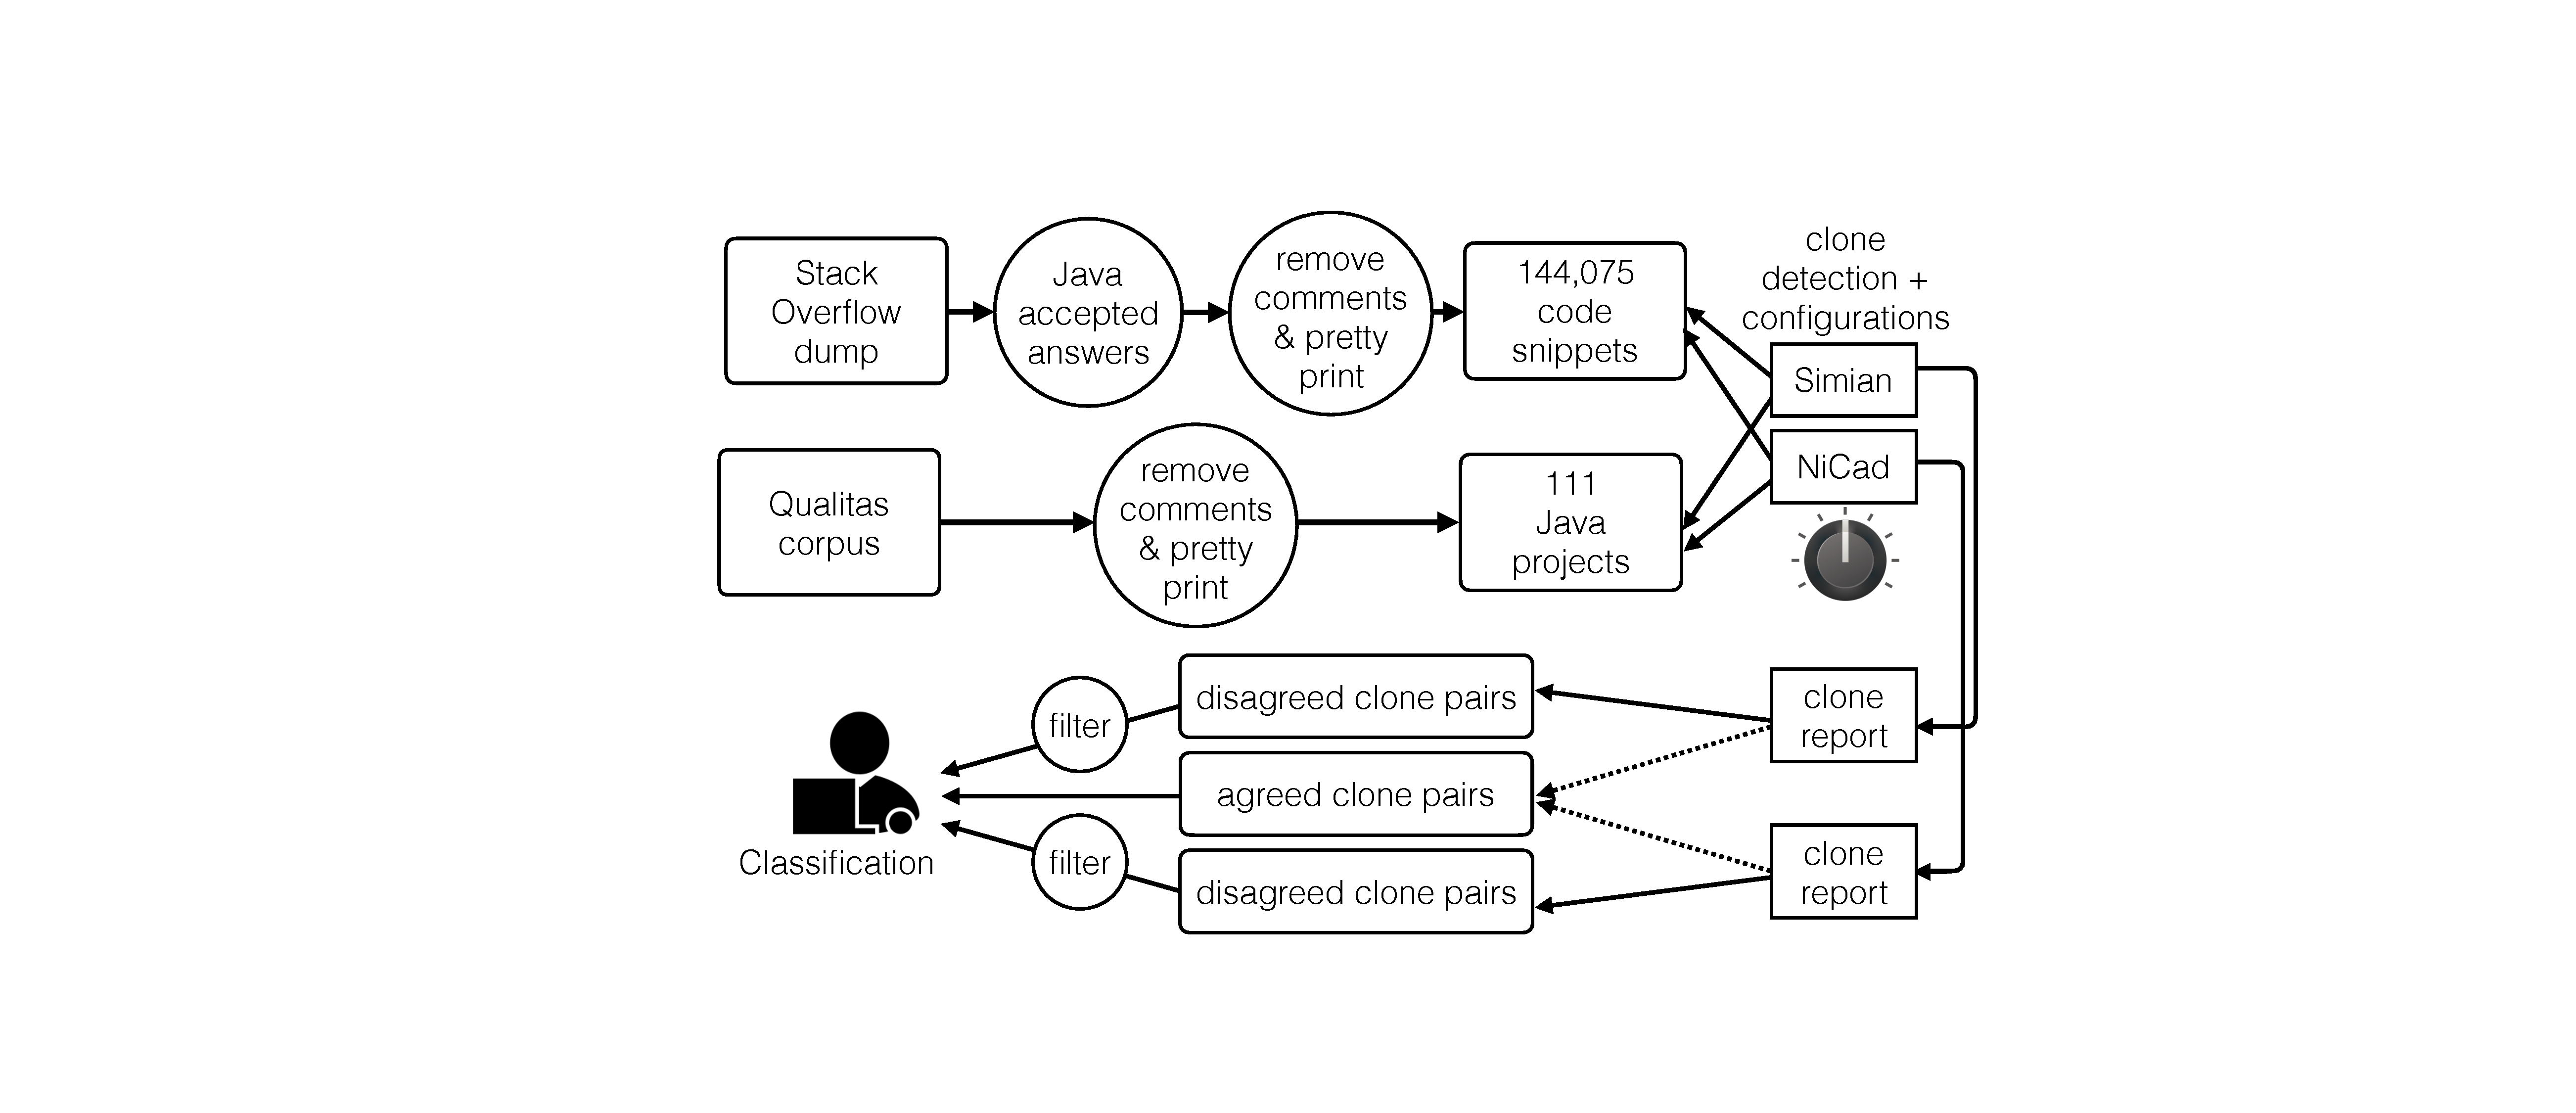
\includegraphics[width=\linewidth]{exp_framework_new}
	\caption{Experimental framework}
	\label{fig:exp_framework}
\end{figure}

\subsection{Experimental Framework}
To answer the four research questions, we followed the experimental framework depicted in \Cref{fig:exp_framework}. We processed two datasets, Stack Overflow and 111 open source projects from Qualitas corpus. Java code snippets were extracted from Stack Overflow posts using regular expressions. We prepared Java code in both datasets by removing comments and pretty-printing to increase accuracy of clone detection. Then, we deployed two clone detection tools, Simian \cite{simian} and NiCad \cite{Roy2008,Cordy}, to locate clones between the two datasets. Due to scalability of Simian and NiCad, we partitioned the input and run the tools multiple times. Each run was composed of the whole Stack Overflow data and single Qualitas project. We repeated the process until we cover 111 projects. 

We then converted the clone reports to General Clone Format (GCF)~\cite{Wang2013} and combined the 111 reports into a single GCF file. GCF provides a common format for clones which enabled us to reuse the same scripts to analyse clone reports from both Simian and NiCad. Moreover, using GCF, other additional clone detectors could be adopted, if needed, without any changes in the analysis. Simian did not provide an option to detect inter clones between two locations. Hence the Simian GCF clone report was pruned to contain only inter clone pairs between Stack Overflow and Qualitas projects. In this step, all intra clone pairs within either Stack Overflow or Qualitas were removed. NiCad provided an option to detect inter clones so no pruning is needed. We did not have an oracle of clones between the two data sets so we rely on a manual investigation to validate the reported clone candidates. However, the large amount of clone pairs hindered us from looking at all of them. Random sampling of clones could be done but may return mostly non-meaningful clones. Instead, we selected clone pair candidates by relying on agreement of clone detectors. If a clone pair was similarly reported by multiple tools, we had a higher confidence that it was a real clone pair. To achieve this, clone pairs from the two clone detectors were pair-wise matched to find agreements using Bellon's clone overlapping criteria \cite{Bellon2007}. This step generated \textbf{agreed clone pairs}. They were pairs with high confidence to be true clones since they obtained agreement from both tools. Then, pairs reported by Simian and NiCad that did not find agreement were \textbf{disagreed clone pairs}. The disagreed clone pairs were clones with less confidence than the agreed ones. Finally, agreed and disagreed clone pairs had been looked at manually by the first and the third author.

In the manual inspection process, we classified clones into seven categories according to information observed from code comments and natural text in Stack Overflow answer. This process took approximately a months until we successfully investigated 3,450 clone pairs. Clone pairs that were classified as false clones, boiler-plate code, or IDE-generated were not very interesting and were ignore in the analysis of outdated code and licensing violation. 
We compared licensing information of 523 remaining clone pairs for possibility of software licensing violations. Moreover, we looked forward through history of each clone from its git repository. With this method, we discovered \textbf{outdated code}, code that changes are made to them after it had been copied to Stack Overflow. %hence resulting in outdated clones on Stack Overflow.

\subsection{Experimental Setup}

\subsubsection{Datasets}

\textbf{Stack Overflow}: we extracted Java code snippets from a snapshot of Stack Overflow dump \footnote{https://archive.org/details/stackexchange} in January 2016. The archived dump has a size of 9 gigabytes. The data dump was in XML format containing information of \textit{Posts} (questions and answers) and supporting data such as user accounts and timestamps of the posts. We were interested in code snippets embedded in posts which were located between \texttt{<code></code>} tags. A Stack Overflow thread contains a post of question and several posts of answers. Every answer has voting score from its users. An answer can also be marked as \textbf{accepted answer} by the questioner if the solution fixes his/her problem. We collected Java code snippets using two criteria. First, we were only interested in code snippets with at least six lines. Snippets which were smaller than six lines were usually spurious clones \cite{Bellon2007}. Second, we only focused on code snippets in accepted answers. We chose the snippets in accept answers because they actually solved the problems in the questions and had a check mark sign on them to notify other users. Moreover, they were always displayed just below the questions which made them attractive to be reused than other answers. Each snippet was extracted from the dump using regular expressions and saved to a file using its post ID as the file's name. If an accepted answer had more than one code snippet, we appended an indexing number, starting from zero, after the post ID (e.g. 45051109\_0, and 45051109\_1.). Lastly, we added \texttt{.java} extension to the file's names so that clone detectors could recognise them. We finally obtained 144,075 Java code snippets which contain 2,347,269 lines of Java source code excluding comments and blank lines\footnote{Measured by cloc: https://github.com/AlDanial/cloc}.

\textbf{Open source systems}: we selected an established corpus for an empirical software engineering study called \textbf{Qualitas} \cite{QualitasCorpus} for this study. It is a curated Java corpus that has been used in several software engineering studies \cite{Taube-Schock2011,Beckman2011,Vasilescu2011,Omar2012}. The projects in the corpus represent various domains of software systems ranging from programming language to 3D and visualisation \cite{QualitasCorpus}. We selected the 20130901r release of Qualitas corpus containing 112 Java open source projects. This release contains projects with releases no later than 1st September 2013. We chose a snapshot late back in 2013 since we are interested in online code clones in the direction from open source projects to Stack Overflow. The 20130901r snapshot provides Java code that is at least 3 years old from the time of the experiment (January to December 2016). The time difference is sufficiently long for a number of code snippets to be copied onto Stack Overflow. Out of 112 Qualitas projects, there is one project, \texttt{jre}, that does not contain Java source code due to its licensing limitation \cite{QualitasCorpus} so it is removed from the study. This resulted in total of 111 projects analysed in the study. As shown in \Cref{tab:datasets}, the 111 Qualitas project have 160,937 Java files containing 19,086,883 lines of code. %Details of the 109 Qualitas projects and their licenses are listed in Table \ref{t:new_and_old}.

\begin{table}
	\centering
	\caption{Stack Overflow and Qualitas datasets}
	\label{tab:datasets}
	\small
	\begin{tabular}{l|r|r}
		\hline 
		Dataset & No. of files & SLOC \\
		\hline
		Stack Overflow & 144,075 & 2,347,269 \\ 
		\hline 
		Qualitas &  160,937 & 19,086,883 \\ 
		\hline 
	\end{tabular} 
\end{table}

\subsubsection{Clone Detectors}
There is a number of restrictions in terms of choosing clone detection tools for this study. First, they have to support Java. Second, due to nature of code snippets posted on Stack Overflow, some of them are not complete Java classes or methods. Hence, the tool must be flexible enough to process code snippets that are neither a complete block nor compilable. Third, since the amount of code that have to be processed are in a scale of millions line of code (as shown in \Cref{tab:datasets}), a clone detector must be scalable enough to successfully complete the execution and report clones in a reasonable amount of time. We have tried running 5 state-of-the-art clone detectors including Simian \cite{simian}, NiCad \cite{Cordy,Roy2008}, CCFinder \cite{Kamiya2002}, iClones \cite{Gode2009}, and DECKARD \cite{Jiang2007a} against Stack Overflow and Qualitas datasets. CCFinder, iClones, and DECKARD failed to report clones between 144,075 Stack Overflow code snippets and 111 Qualitas projects. All of them reported execution errors after running for couple of hours. Thus, we removed them from the study. Simian and NiCad completed the detection with success. We found that both of them are also flexible enough to handle code with incomplete methods or classes. %So, we decided to use both of them.

\textbf{Simian} is a text-based clone detector which locate clones at line-level granularity and has been used extensively in several clone studies \cite{Ragkhitwetsagul2016, Wang2013, Mondal2011, Cheung2015, Krinke2010}. It is a command-line tool which enables us to automate the detection. Furthermore, it offers normalisation of variable names and literals (strings, and numbers) which enable Simian to detect literal clones (type-1) and parameterised clones (type-2). \textbf{NiCad} is also a text-based clone detector which detects clones at either method- or block-level granularity. It can detect clones of type-1, 2 up to type-3 (clones with added/removed/relocated/changed statements) and is also used in several empirical clone studies \cite{Roy2008, Ragkhitwetsagul2016, Svajlenko2014, Wang2013, Mondal2011, Sajnani2016}. It utilises TXL \cite{Cordy2006} for parsing and pretty-printing source code. It also provide code normalisation by variable renaming and abstraction. We use a variant of NiCad called \textit{nicadcross}. It offers the same functionalities as the original NiCad but is specialised for detecting code clones between two systems. NiCad is also a command-line tool which makes it suitable for automation.

\subsubsection{Prioritise Clone Candidates Using Agreement}
A number of clones detected in large-scale datasets can be huge. In our study, there are totally 266,837,480 clone pairs reported. It is almost infeasible for human to manually validate them all. One can do a random sampling of clones. However, due to a very high number of false positives, they may end up looking at most of the false clones. Therefore, we adopted an idea of \textbf{clone agreement} which has been used in clone research studies \cite{Wang2013,Funaro2010,cr2016ssbse} in a situation that clone oracle is missing or impossible to establish. Clone pairs agreed by multiple clone detection tools have higher confident to be real clones \cite{cr2016ssbse}. By using this agreement-based approach, we could reduce the number of clone candidates for manual investigation by paying more attention to the ones agreed by multiple tools. To find an agreement between two clone pairs report by two different tools, we used clone pair matching metric proposed by Bellon et al.~\cite{Bellon2007}. Two clone pairs which have large enough overlapping clone lines can be categorised as either a good-match or an ok-match pair (denoted as \textit{good} and \textit{ok} respectively) with a confident value between 0 and 1. A \textit{good} clone pair has stronger agreement than an \textit{ok} pair. We follow the following definitions of good- and ok-match introduced in the original paper.

\vspace{0.5ex}
Given that a clone pair \textit{CP} is formed by two clone fragments \textit{CF$_1$} and \textit{CF$_2$} with a pre-defined similarity threshold \textit{t}, i.e.~\textit{CP} = (\textit{CF$_1$}, \textit{CF$_2$}, \textit{t}), we can define \textit{overlap} and \textit{contained} value of two clone pairs as 
%\squeezeup
\begin{multline}
	overlap(\textrm{\textit{CP}}_1, \textrm{\textit{CP}}_2) = \frac{|lines(\textrm{\textit{CF}}_1) \cap lines(\textrm{\textit{CF}}_2)|}{|lines(\textrm{\textit{CF}}_1) \cup lines(\textrm{\textit{CF}}_2)|} 
\end{multline}
%\squeezeup
\begin{multline}
	contained(\textrm{\textit{CP}}_1, \textrm{\textit{CP}}_2) = \frac{|lines(\textrm{\textit{CF}}_1) \cap lines(\textrm{\textit{CF}}_2)|}{|lines(\textrm{\textit{CF}}_1)|}. 
\end{multline}

\noindent\textit{good-value} of two clone pairs is then defined as
%\squeezeup
\begin{align*}
	good(\textrm{\textit{CP}}_1, \textrm{\textit{CP}}_2) = min(overlap(\textrm{\textit{CP}}_1.\textrm{\textit{CF}}_1,\textrm{\textit{CP}}_2.\textrm{\textit{CF}}_1), \\ overlap(\textrm{\textit{CP}}_1.\textrm{\textit{CF}}_2,\textrm{\textit{CP}}_2.\textrm{\textit{CF}}_2)).
\end{align*}

\noindent\textit{ok-value} is defined as
%\squeezeup
\begin{align*}
	ok(\textrm{\textit{CP}}_1,\textrm{\textit{CP}}_2) = min(max(contained(\textrm{\textit{CP}}_1.\textrm{\textit{CF}}_1,\textrm{\textit{CP}}_2.\textrm{\textit{CF}}_1), \\ contained(\textrm{\textit{CP}}_2.\textrm{\textit{CF}}_1,\textrm{\textit{CP}}_1.\textrm{\textit{CF}}_1)),
	\\ max(contained(\textrm{\textit{CP}}_1.\textrm{\textit{CF}}_2,\textrm{\textit{CP}}_2.\textrm{\textit{CF}}_2), \\contained(\textrm{\textit{CP}}_2.\textrm{\textit{CF}}_2,\textrm{\textit{CP}}_1.\textrm{\textit{CF}}_2))).
\end{align*}

Two clone pairs $\textrm{\textit{CP}}_1$ and $\textrm{\textit{CP}}_2$ are called a \textit{\textit{good}(p)} iff, for $p \in [0,1]$ holds 
%\squeezeup
\begin{equation}
good(\textrm{\textit{CP}}_1,\textrm{\textit{CP}}_2) \geq p.
\end{equation}

Similarly for an \textit{ok-match(p)} pair
%\squeezeup
\begin{equation}
ok(\textrm{\textit{CP}}_1,\textrm{\textit{CP}}_2) \geq p.
\end{equation}

Using this good and ok-match criteria with a predefined threshold \textit{p}, we can prune the 266-million candidate clone pairs for manual investigation. \textit{good} pairs are the ones with the highest confident and ranked the first to be looked at, followed by \textit{ok} pairs, and followed by clone pairs without agreement.

\subsection{Clone Detector's Parameter Tuning}
We were aware of effects of configurations to clone detection results and the importance of searching for optimised configurations in empirical clone studies \cite{Wang2014,cr2016ssbse,Ragkhitwetsagul2016,Svajlenko2014}. However, considering the massive size of the two datasets and search space of at least 15 Simian's and 5 NiCad's parameters, we were hindered from searching for the best configurations of the tools. Thus, we decided to configure Simian and NiCad using two established configurations: 1) the tools' default configurations chosen by the tools' creators (denoted as \textit{D}), and 2) the discovered configurations for Bellon's Java projects from \textit{EvaClone}, a study of optimising clone detectors' configurations based on clone agreement, by Wang et al.~\cite{Wang2013} (denoted by \textit{E}). The details of the two configurations are described in \Cref{t:param_tuning}. Having two clone detectors, Simian (denoted as \textit{S}) and NiCad (denoted as \textit{N}), with two chosen configurations each, we looked for Bellon's good and ok-match in four possible pair-wise combinations: $S_{D}N_{D}$, $S_{D}N_{E}$, $S_{E}N_{D}$, and $S_{E}N_{E}$.

\begin{table}
	\centering
	\caption{Configurations of Simian and NiCad}
	\label{t:param_tuning}
%	\resizebox{\columnwidth}{!}{%
	\small
	\begin{tabular}{l|p{7cm}}
		\hline 
		Tool & Parameters \\
		\hline
		$S_D$ &  threshold=6, ignoreStringCase, \newline ignoreCharacterCase, ignoreModifiers \\ 
		\hline
		$S_E$ & threshold=5, ignoreIdentifiers, \newline ignoreIdentifierCase, ignoreStrings, \newline ignoreCharacters, ignoreSubtypeNames, \newline balanceSquareBrackets  \\ 
		\hline 
		$N_D$ & Blocks, MinLine=10, MaxLine=1000, UPI=0.30 \\
		\hline
		$N_E$ & Blocks, MinLine=5, MaxLine=604, UPI=0.20, \newline blind renaming, literal abstraction \\ 
		\hline 
	\end{tabular} %
%}
\end{table}

\section{Results and Discussion}

We followed the experimental framework and detected clones between Stack Overflow and Qualitas corpus using the two selected clone detectors. To answer RQ1, we computed statistics of clone discovered by the tools. To answer RQ2, we manually investigated online clone pair candidates and categorised them using our patterns of online code cloning. The patterns were derived from Kapser et al.~\cite{Kapser2003} augmented by common patterns found in our data set. For RQ3, we looked at the true positive clone pairs and check if they are still up-to-date. Similarly, for RQ4, we also looked at the license of each clone and observed a possibility of licensing violation.

\subsection{RQ1: Online Code Clones} 

\begin{table}
	\centering
	\caption{Statistics of clones found between Stack Overflow and Qualitas projects using Simian (\textit{S}) and NiCad (\textit{N}) with default (\textit{D}) and EvaClone (\textit{E}) configurations \FIXME{boxplots here?}}
	\label{tab:raw_stats}
	\small
	\resizebox{\columnwidth}{!}}}$ & 29\% & 28\% & 25\% & 21\% \\
			\hline
		\end{tabular} %
	}
\end{table}

The clone statistics obtained from running Simian and NiCad with \textit{D} and \textit{E} configurations are presented in \Cref{tab:raw_stats}. From \Cref{tab:raw_stats}, Simian clones cover approximately 1\% of the 144,075 Stack Overflow snippets, 1,086 reported by $S_D$ and 1,531 from $S_E$ respectively. $N_D$ reports clones in 1,392 Stack Overflow code snippets, while $N_E$ reports clones in a larger number of 12,886 snippets  mainly due to its relaxed configurations. In terms of number of clone pairs, $S_E$ and $N_E$ report a large number of clone pairs of 63,635,844 and 251,449,849 respectively. This is expected since EvaClone configurations prefer recall so it tends to remote more clones \cite{Wang2013}. The average clone size of $S_D$ is 7.72 lines which is bigger than its $S_E$ counterpart of 4.79. Similarly, $N_D$ has an average clone size of 9.84 lines which is bigger than 5.33 reported by $N_E$. We can see from the statistics that EvaClone tunes the tools in the way that they report smaller clones. The average percentage of Stack Overflow code snippets that are cloned according to $S_D$, $S_E$, $N_D$, and $N_E$ is 29\%, 28\%, 25\%, and 21\% accordingly. A quick manual check of Simian's clone report revealed that there were problematic 11 snippets. These 11 snippets triggered Simian to generate large clone clusters containing a huge number of false clones from array initialisation. Hence, their clones were removed from further analyses. 

As displayed in \Cref{tab:online_clone_pairs}, after we applying clone agreement filtering using Bellon's criteria, the number of \textit{good} agreed clone pairs is 2,308 while \textit{ok} is 11,749. The number of disagreed clone pairs ($S_D$, $N_D$) after filtering is 17,801 and 181 for Simian and NiCad respectively. The total number of clone candidates is 32,039 pairs. The details are as follows.

\begin{table}
	\centering
	\caption{The number of online clone pair condidates (mutually exclusive) before and after filtering.}
	\label{tab:online_clone_pairs}
	\small
%	\resizebox{\columnwidth}{!}{%
	\begin{tabular}{l|r|c|c|c|c|r}
		\hline
		\multirow{2}{*}{Set} & \multicolumn{1}{c|}{Before} & \multicolumn{4}{c|}{Filters*} & \multirow{2}{*}{Cand.} \\ \cline{3-6}
		& \multicolumn{1}{c|}{Filters} & \textit{L} & \textit{S} & \textit{R} & \textit{G} & \\
		\hline 
		\multirow{1}{*}{\textit{good}} & 2,308 & & & & & 2,308 \\
		\multirow{1}{*}{\textit{ok}} & 11,749 & & & & & 11,749 \\
		%\multirow{1}{*}{\textit{agreed clone pairs}}      & 29,099 \\
		\multirow{1}{*}{$S_D$} & 67,570 & \checkmark & & \checkmark & \checkmark & 17,801 \\
		\multirow{1}{*}{$N_D$} & 229,176 & & \checkmark & \checkmark & \checkmark & 181 \\ 
		%\multirow{1}{*}{\textit{disagreed clone pairs}}    & 1,039 \\
		\hline
		Total  & 310,803 & & & & & 32,039 \\ 
		\hline
		\multicolumn{7}{l}{\scriptsize{Filters*: \textit{L}=$Line \geq 10$, \textit{S}=$Sim \geq 85\%$,}} \\
		\multicolumn{7}{l}{\scriptsize{\textit{R}=regular expressions, and \textit{G}=\textit{good}/\textit{ok} pairs.}} \\
	\end{tabular} %
%}
\end{table}

\begin{table}
	\centering
	\caption{The online clone classification results}
	\label{tab:online_clone_classification_results}
	\small
	%	\resizebox{\columnwidth}{!}{%
	\begin{tabular}{l|r|r|r|r}
		\hline
		\multirow{2}{*}{Set} & \multirow{2}{*}{Candidates} & \multicolumn{2}{c|}{Classification} & \multirow{2}{*}{TP} \\ \cline{3-4}
		& & Auto & Manual & \\
		\hline 
		\multirow{1}{*}{\textit{good}} & 2,308 & 9 & 2,299 & x \\
		\multirow{1}{*}{\textit{ok}} & 11,749 & 11,495 & 254 & x \\
		%\multirow{1}{*}{\textit{agreed clone pairs}}      & 29,099 \\
		\multirow{1}{*}{$S_D$} & 17,801 & 16,930 & 871 & 704 \\
		\multirow{1}{*}{$N_D$} & 181 & 10 & 171 & x \\ 
		%\multirow{1}{*}{\textit{disagreed clone pairs}}    & 1,039 \\
		\hline
		Total  & 32,039 & 28,444 & 3,595 & x \\ 
		\hline
	\end{tabular} %
	%}
\end{table}

\subsubsection{Agreed clone pairs}

Agreed clone pairs are clone pairs that pass Bellon's good- or ok-match criteria and selected for manual investigation. Similar to the original study, we select a threshold \textit{p} of 0.7 for both \textit{good} and \textit{ok} pairs \cite{Bellon2007}. %The number of projects processed by the clone detection tools are listed in \Cref{tab:projects_missing}. 
We encountered NiCad failures with a few Qualitas projects.~$N_D$ could not detect clones in \texttt{hibernate} due to clustering errors. $N_E$ generated renaming errors for 5 projects including \texttt{vuze}, \texttt{hibernate}, \texttt{myfaces}, \texttt{netbeans}, and \texttt{spring}. We had contacted the creator of NiCad regarding the issues. They identified them as problems of long file paths and TXL grammars which will be fixed in the next NiCad releases. As a result, we did not have NiCad clones from these projects in the agreed clone pairs. Simian clones of the same projects also disappeared from the agreed clone pairs since they could not find matches.

\begin{table}
	\centering
	\caption{Distribution of the agreed clone pairs}
	\label{t_agreed_good_clone_pairs}
	\small
	\resizebox{\columnwidth}{!}{%
	\begin{tabular}{l|r|r|r|r|r|r}
		\hline
		Set & $S_DN_D$ & $S_DN_E$ & $S_EN_D$ & $S_EN_E$ & Total & Unique \\
		\hline
		\textit{good} & 18 & 26 & 10 & 2,267 & 2,321 & 2,308 \\
		\textit{ok} & 11,467 & 993 & 79 & 20,021 & 32,560 & 31,729  \\
		\hline
	\end{tabular} %
}
\end{table}

\begin{figure}
	\centering
	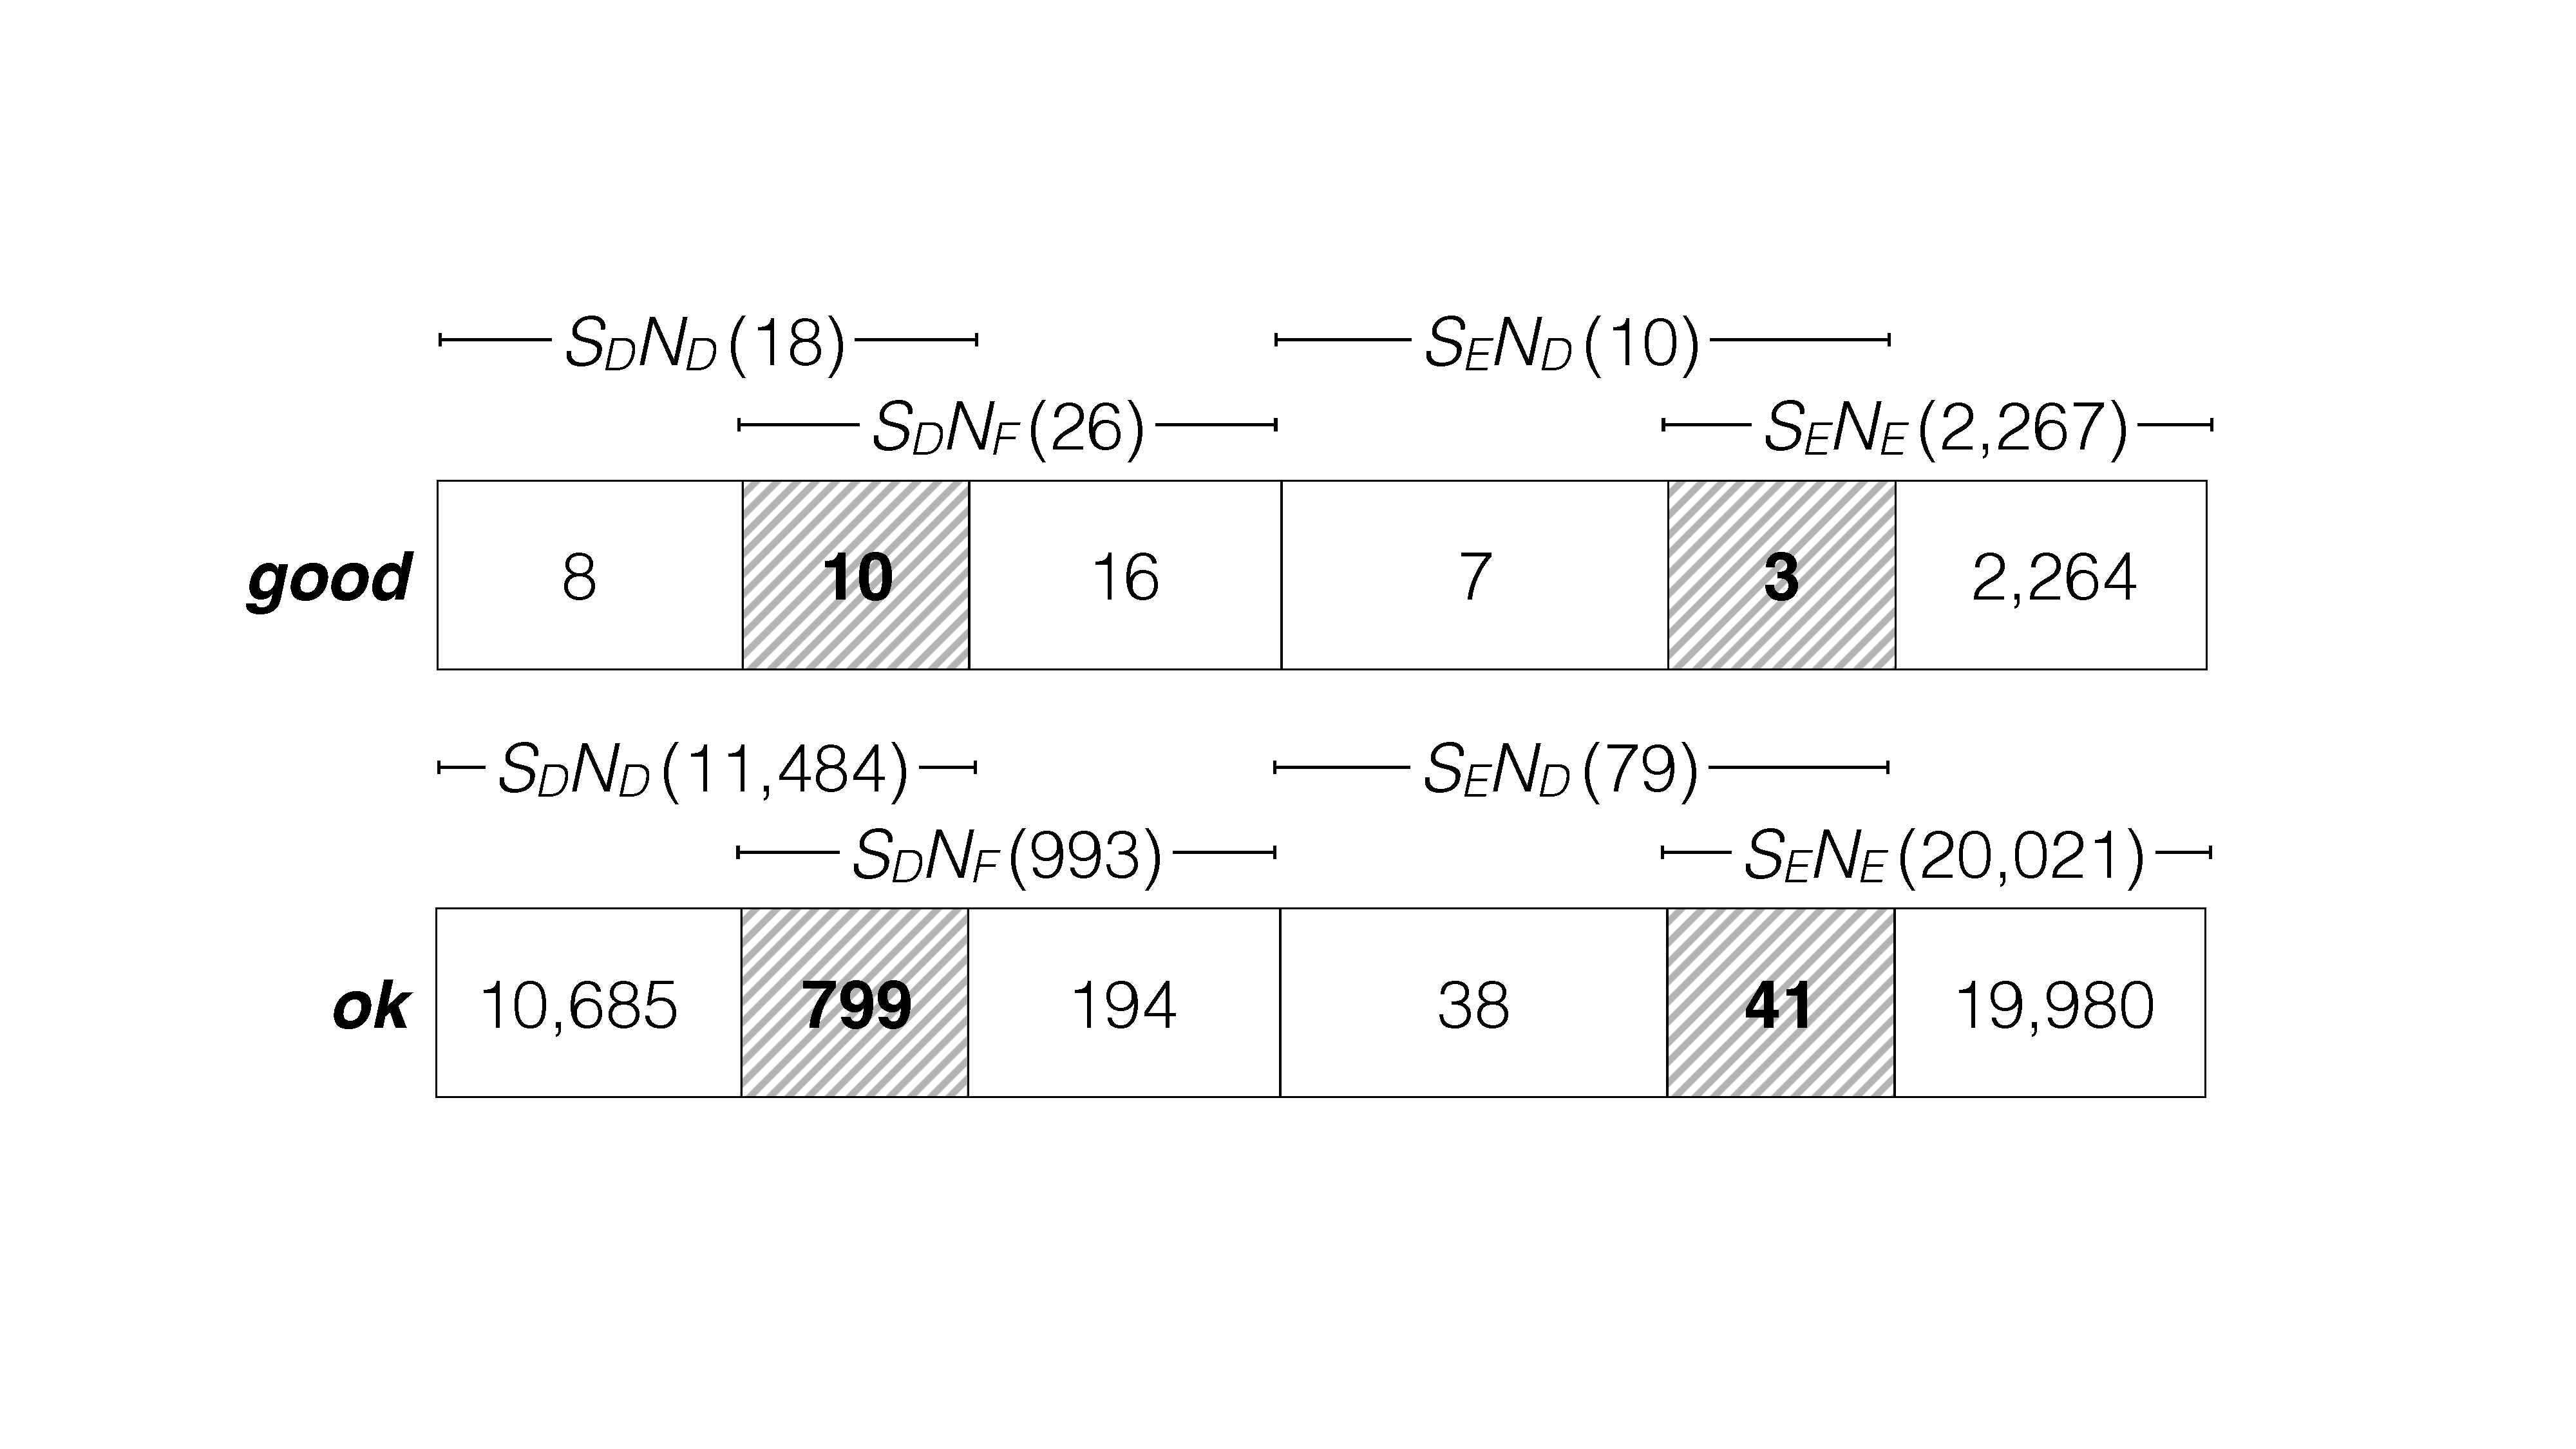
\includegraphics[width=\linewidth]{good-ok_pairs-crop}
	\caption{Distribution of \textit{good} (top) and \textit{ok} pairs (bottom) in 4 configurations of Simian and NiCad. The shaded areas are overlapping pairs.}
	\label{fig:good-ok-pairs}
\end{figure}

The distributions of \textit{good} clone pairs between four combinations of \textit{D} and \textit{E} configurations are listed in \Cref{t_agreed_good_clone_pairs} and depicted visually in \Cref{fig:good-ok-pairs}. There are 2,321 (2,308 unique) \textit{good} pairs consisting of 18 pairs from $S_DN_D$, 26 pairs from $S_DN_E$, 10 pairs from $S_EN_D$, and 2,267 pairs from $S_EN_E$. There are 32,560 (11,749 unique) \textit{ok} pairs\footnote{This excludes the subsumed 2,308 \textit{good} pairs. According to the definition, \textit{ok} pairs always subsume \textit{good} pairs.} We obtained 11,467; 993; 79; and 20,021 pairs from $S_DN_D$, $S_DN_E$, $S_EN_D$, and $S_EN_E$ respectively. Between the four configuration sets, there are considerable amount of clone pairs shared between two adjacent sets (as depicted in \Cref{fig:good-ok-pairs}), but there is no clone pair that is agreed by all four combinations. 

\subsubsection{Disagreed clone pairs}

The disagreed clone pairs are clone pairs that are reported by a single tool, either Simian or NiCad, and do not have agreement with clones from another tool. The disagreement can be from misalignment of clone lines or totally dissimilar clones due to different configurations. Disagreed pairs from Simian also cover clone pairs in projects having NiCad's errors (1 projects for $N_D$ and 5 for $N_E$) that are automatically missing from the agreed clone pairs. With the four configuration combinations, we decided to investigate only $S_D$, and $N_D$, and drop $S_E$ and $N_E$ due to their enormous amount of clone pairs (60 and 250 millions respectively). Moroever, without clone agreement, $S_E$ and $N_E$ contain a large number of false positives due to the recall preference of their EvaClone configurations. 

Even choosing only the default configurations, the number of clone pair candidates are still very large for manual inspection (67,570 for $S_D$ and 229,176 pairs for $N_D$). We hence apply four filters: \textbf{clone size, regular expression, similarity threshold, and good/ok pairs}. For the clone size filter, we raise the minimum clone size to 10 line as larger clones tend to be more interesting while smaller ones tend to be false clones \cite{Saini2016}. Moreover, Gabel and Su show that unique code tend to be larger than seven lines \cite{Gabel2010}. The 10--line threshold is already the default configuration for NiCad, thus this filter affects Simian clones only (Simian's default configurations consider a minimum of 6 lines).~The regular expression filter captures uninteresting boiler-plate clones of \verb|hashCode()| methods and some of the obvious getters and setters using regular expressions and removes them. The third filter, similarity threshold, applies only to NiCad clone pairs since Simian does not provide this similarity threshold configuration. The last filter, good/ok pairs, filters the pairs that already exist in \textit{good} or \textit{ok} set to avoid duplicates. 

As shown in \Cref{tab:online_clone_pairs}, for $S_D$ we filtered the results using clone size, regular expressions, and gook/ok pairs. The combination of the three filters reduce the number of $S_D$ clones to 17,801 pairs for manual investigation. 
For $N_D$, 10-line threshold is already a minimum NiCad's clone size. However, NiCad still reported much more clone pairs than Simian since it can detect type-3 clones. Thus, besides regular expressions and good/ok pair filters, we filtered NiCad's clones further by a stricter similarity threshold. We increase NiCad's similarity threshold from 70\% to 85\% (by adjusting NiCad's $\mathrm{UPI}$ from 0.3 to 0.15). We have tried varying the UPI from 70\% (default), 80\%, 85\% and 90\% and we found that 85\% similarity provides the best balance in terms of the amount of reported clones and feasibility for manual investigation. Using the three filters, we reduced the size of $N_D$ clones to 181 pairs.

In our clone classification process, we used a script to automatically classify \texttt{equals()} clone pairs which helped classifying 28,444 pairs out of 32,039 (more than half of the \texttt{equals()} pairs came from \textit{ok} and $S_D$ pairs). Finally, there are 3,595 pairs remaining which we manually classified them. The classification summary is shown in \Cref{tab:online_clone_classification_results}.

\textbf{To answer RQ1, we found 32,039 clone candidates between 111 Qualitas projects and 144,075 Stack Overflow snippets. They are 2,308 \textit{good}, 11,749 \textit{ok}, 17,801 $S_D$, and 181 $N_D$ pairs. After classification, we found at least \FIXME{NUMBER} online code clones pairs between Stack Overflow and Qualitas.}

%We selected only Stack Overflow fragment and Qualitas files that have never been looked at before in the previous investigation. If many clone pairs having the same Stack Overflow fragment and Qualitas file, we keep only the largest one. The reason for having this criteria is that we found a lot of duplicate clone pairs with the same classifications from either Stack Overflow fragments or Qualitas files. The classification results are shown in Table \ref{tab:classification_indv}. 

%\begin{table}
%	\centering
%	\caption{No.~of disagreed clone pairs ($S_D$ and $N_D$).}
%	\label{tab:classification_indv_stats}
%	\small
%	\resizebox{\columnwidth}{!}{%
%	\begin{tabular}{l|p{1.6cm}|r|r|r|r}
%		\hline 
%		Tool & Filter & \multicolumn{1}{c|}{Original} & \multicolumn{1}{c|}{Filtered} & \multicolumn{1}{c|}{good/ok} & \multicolumn{1}{c}{remaining} \\ 
%		%\hline 
%		%\multirow{1}{*}{\textit{Simian$_{df}$}-1} & 9383 & 140 & 8951 & 292 \\
%		%\multirow{1}{*}{\textit{Simian$_{df}$}-2} & 9042 & 0 & 8539 & 503 \\
%		\hline
%		\multirow{1}{*}{\textit{Simian$_{df}$}} & $Line \geq 10$ \newline \& RegEx & \multirow{2}{*}{67,570} & \multirow{2}{*}{47,223}  & \multirow{2}{*}{2,546} & \multirow{2}{*}{17,801} \\ %140 + 1482 + 926
%		\hline
%%		\multirow{1}{*}{\textit{$N_D$}-1} & 7040  & 226 & 6700 & 114 \\
%%		\multirow{1}{*}{\textit{$N_D$}-2} & 22187  & 152 & 21990 & 45 \\
%		\multirow{1}{*}{\textit{$N_D$}} & $Sim \geq 80\%$ \newline \& RegEx & \multirow{2}{*}{229,176} & \multirow{2}{*}{228,558}  & \multirow{2}{*}{450} & \multirow{2}{*}{168} \\
%		\hline
%		%\multicolumn{2}{l|}{Total} & 296,746 & 20,966 & 2,996 & 1,039 \\
%		%\hline
%	\end{tabular} %
%	}
%\end{table}

\subsection{RQ2: Patterns of Online Code Cloning}

\begin{table}
	\centering
	\caption{Seven patterns of online code cloning}
	\label{tab:classification_scheme}
	\resizebox{\columnwidth}{!}{%
		\begin{tabular}{c|p{8.4cm}}
			\hline 
			Patt. & Descriptions \\ 
			\hline 
			QS & Cloned from Qualitas project to Stack Overflow (Q $\rightarrow$ S). \\ 
			\hline 
			SQ &Cloned from Stack Overflow to Qualitas project (S $\rightarrow$ Q). \\ 
			\hline 
			UD & Cloned from each other or from an external source \textit{X} outside the project (unknown) (S $\leftrightarrow$ Q $\vee$ (X $\rightarrow$ S $\wedge$ X $\rightarrow$ Q)).
			\\ 
			\hline 
			ES & Cloned from an external source (X $\rightarrow$ S $\wedge$ X $\rightarrow$ Q).
			\\ 
			\hline 
			BP & Boiler-plate or IDE auto-generated
			\\ 
			\hline 
			IN & Inheritance, interface implementation 
			\\ 
			\hline 
			FC & Accidental similarity, false clones \\ 
			\hline 
		\end{tabular}  %
	}
\end{table}

Besides the quantitative analysis, we are also interested in a qualitative analysis of the online clones. How are the clone pairs created? %Due to an absence of clone oracle of the two data sets, we resort to a manual investigation to classify the clone pair candidates using our 7 patterns of online code cloning.  

We started by a preliminary study of the 8 patterns of cloning from Kapser et al.~\cite{Kapser2006,Kapser2008}. This preliminary investigation aims to evaluate the applicability of Kapser's cloning patterns to our study. Using $S_D$ clone report, snippets are ranked according to (1) frequency, (2) popularity (i.e.~number of associated Qualitas projects), (3) clone size in SLOC, and (4) clone percentage compared to the snippet size. We selected these criteria so that we can cover clones across various aspects. We then picked the top 10 snippets from the 4 groups resulting in 34 unique Stack Overflow snippets chosen. The 34 snippets generate 697 clone pairs with Qualitas projects. Using Kapser's cloning patterns, the clone pairs were categorised into either Customisation or Templating. \textbf{Clearly Kapser's cloning patterns are too broad for our study and a more suitable and fine-grained classification scheme is needed.} 

Nevertheless, we adopted one of Kapser's cloning patterns, boiler-plate code and API/library protocol as pattern BP. We then added 6 new patterns observed as common cloning patterns from our preliminary study. The seven patterns include QS, SQ, UN, ES, BP, IN, and FC as presented in \Cref{tab:classification_scheme}. QS (\textbf{Q}ualitas to \textbf{S}tack Overflow) represents clones that has evidence to be copied from Qualitas to Stack Overflow (by having comments in source code and explanation/links in Stack Overflow post). Pattern SQ (\textbf{S}tack Overflow to \textbf{Q}ualitas) is the opposite of QS. UD (\textbf{U}nknown \textbf{D}irection) is cloning that creates exactly identical or highly similar clones but without any attribution of copying. They are unique enough not be boiler-plate and inheritance or interface implementation. ES (\textbf{E}xternal \textbf{S}ources) is a cloning that has an evidence of copying from an external source(s). Pattern BP (\textbf{B}oiler-\textbf{P}late) represents clones containing boiler-plate code of \verb|equals()| methods, getters and setters, or IDE-generated code (e.g.~GUI components). Pattern IN (\textbf{In}heritance/Interface) is cloning because of inheritance of the same super class or implementation of the same interface. They usually share similar overriding methods. The last pattern, FC (\textbf{F}alse \textbf{C}lones), represents false clone pairs. They can be either accidentally similar clones (e.g.~similar \texttt{try-catch} statements), similar clones after code normalisation, or just false positives of the tools. Using the classification patterns, we can also calculate the number of true and false positives. We are looking for unique and meaningful clones in this study. Thus, we consider clone pairs classified into pattern QS, SQ, and UN as true positive, and BP, IN, and FC as false positive.

\subsubsection{Classification of Clone Candidates}

There were 32,039 online clone pair candidates for classifications as shown in \Cref{tab:online_clone_pairs}. We have use regular expressions to automatically classify \texttt{equals()} methods based on the method signature since they are not very interesting clones. It captured 28,444 clone pairs and classified them into pattern D. With help of the automatic classification, there were 3,595 pairs left for manual classification.

The first author who has been working on clone detection research for two years took the role of a main investigator performing a manual classification of all the 3,595 clone pairs. By consulting the cloning patterns, the main investigator manually went through each clone pair candidate, looked at the clones, and chose the most appropriate cloning pattern for the pair. A relevant and useful observation was also recorded for each clone pair. The second author took the role of a validating investigator performing 10\% validation (359 pairs) of the clone pairs judged by the main investigator. The two investigators discussed 54 classification conflicts and resolved 51 of them. The 3 conflicts which the two investigators could not find consensuses are resolved after involving the third author. 

The classification results are shown in \Cref{tab:classification_good_o}. For \textit{good} pairs, 9 pairs were automatically classified by regular expressions and 2,299 pairs were manually classified. This resulted in one clone pair in pattern QS which is found to be copied from a Qualitas project to Stack Overflow. Four pairs are highly similar or identical but without any evidence of copying (no comments in neither Stack Overflow post nor Qualitas source code) and are classified as pattern UD. We observed 3 pairs in pattern ES since they are copied from external sources. 58 clone pairs are found to be pattern BP. Six pairs are similar code from inheriting the same superclass or implementing the same interface, pattern IN. Finally, 2,189 pairs are false clones and classified into FC. No clones were found in pattern SQ. This was expected since we selected a pretty old Qualitas snapshot dated back 2013 and most of the code could be written long before that.  

For the \textit{ok} clone pairs, we could not feasibly investigate all 31,729 pairs manually.  Consulting the classification of \textit{good} pairs, we found that $S_EN_E$ produces a large number of x,xxx false positive results (accounts for xx.xx\% of $S_EN_E$ clone pairs) due to its recall preference. We thus decided to ignore this clone set in our \textit{ok}-pair classification. A large number of 11,495 clone pairs were automatically classified and 254 pairs were done manually. We found xx, xx, xx, xx, xx, and xx in QS, UD, ES, BP, IN and FC respectively. Similarly, no clone pairs were found in SQ. 

\begin{table}
	\centering
	\caption{Classification results of agreed and disagreed clone pairs.}
	\label{tab:classification_good_o}
	\small
	\resizebox{\columnwidth}{!}{%
		\begin{tabular}{l|r|r|r|r|r|r|r|r}
			\hline
			Set & A & A' & B & C & D  & E & F & Total \\ 
			\hline
			\multirow{1}{*}{\textit{good}}  & 1 & 0 & 4  & 3 & 58  & 6 & 2,189 & 2,261 \\
			\multirow{1}{*}{\textit{ok}}  & 8 & 0 & 29  & 10 & 9,158 & 35 & 82 & 9,322 \\
			\multirow{1}{*}{$S_D$} & 79 & 0 & 336 & 17 & 209 & 63 & 167 & 871 \\
			\multirow{1}{*}{$N_D$} & 8  & 0 & 27 & 1 & 77 & 3 & 82 & 168 \\ 
			\hline
			Total & 96 & 0 & 396 & 31 & 9,502 & 107 & 2,520 & 12,622 \\ 
			\hline
		\end{tabular} 
	}
\end{table}

For disagreed clone pairs, an automatic and manual classification of 17,801 $S_D$ and 181 $N_D$ clone pairs results in xx pairs in pattern QS, xx pairs in UD, xx pairs in ES, xx in BP, xx in IN and xx in FC. 

\textbf{To answer RQ2, we found that ...}

\subsection{RQ3: Outdated Online Code Clones}

%In this study, we are interested in effects of having code clones between open source software systems and Stack Overflow. From the manual investigation, we found 523 true positive online clone pairs. With this set of true clones, we investigated further and found that there are two potential issues, outdated code and software licensing violation.

%\subsubsection{Outdated Clones}
Outdated code occurs when a piece of code has been copied from its origin to another location and later the original code has been updated \cite{Xia2014}. Usually code clone detection is used to locate clone instances and update them to match with the original code \cite{Bellon2007}. However, in this situation, the clones are pervasive on Stack Overflow posts and are more difficult to detect than in a local project(s) due to its large search space and the mix of natural and programming language combined together in Stack Overflow posts. Moreover, Stack Overflow is not a software. There is no test suite to run and check whether the code snippets are still working as expected. Hence, if any change happens in the original code, our results show that the copies on Stack Overflow are still mostly left outdated. 

As far as we know, our work is possibly the first which discovers outdated code on Stack Overflow. Since code can be updated due to various possible reasons, e.g.~bug fixing or API changes, it is risky if developers reuse outdated code snippets from Stack Overflow.
They might later find out that the copied code does not work any more due to different API versions. Even worse, they might also introduce bugs or vulnerabilities into their software. 

To check if the discovered Stack Overflow clones are outdated, we focused on the 96 QS clone pairs that are copied in the direction from Qualitas to Stack Overflow (see \Cref{tab:classification_good_o}). For each code snippet, we tracked its original code in Qualitas projects. We located the latest version of the each file and compared to the Stack Overflow snippet to see if any change has been made to the source code. If we found any change, we used \textit{git blame} command to see who modified the source code and when.

\Cref{fig:outdated} shows the findings of outdated online clones on Stack Overflow. The comparison with the clones' latest versions revealed that 55 clone pairs were outdated and they were all Stack Overflow accepted answers. \texttt{hadoop} and Spring have the maximum number of 9 outdated code clones, followed by 6 from Tomcat, and 5 from \texttt{eclipse-SDK}. An example of outdated code in \texttt{hadoop}'s \textit{WritableComparator.java} is shown in \Cref{fig:before-after} as we discussed before. We also found a few outdated code which contained heavy modifications. For example, the code snippet in Stack Overflow post 23520731, a copy of \textit{SchemaUpdate.java} in \texttt{hibernate}, it had been heavily modified in the latest version (as shown in \Cref{fig:hibernate_outdated_code}). Lastly, we found some ``orphan'' snippets. These snippets cannot find their originals in the latest version of the projects anymore. For example, the snippet in Stack Overflow post 3758110, a copy of \textit{DefaultAnnotationHandlerMapping.java} in \texttt{spring}, was deleted in commit \texttt{02a4473c62d8240837bec297f0a1f3cb67ef8a7b} by Chris Beams on 20th January 2012 at 22:51:02, two years after it was posted. %The latest version of Spring does not contain the file anymore. 

The outdated online code clones can cause problems ranging from uncompilable code due to different API usage to bug propagations. An outdated code with a subtle change (e.g.~\Cref{fig:before-after}) may be copied and reused without awareness from developers. Although Stack Overflow has a voting mechanism that may mitigate this outdated code issue, the check mark symbol in front of the accepted answer is still attractive to naive developers who are ignorant.

\textbf{For RQ3, we found 55 code snippets on Stack Overflow that are outdated and questionable for being reused.}
%Usually when developers reuse a code snippet from a Stack Overflow post and find that it does not work nor compatible with their environment. They can cast a down vote to that answer resulting in low votes for the answer (which might be outdated). However, if the answer is marked as accepted by the person who asks the question, the check mark symbol attached to the answer is still attractive to naive developers who are ignorant. 

\begin{figure*}
	\begin{lstlisting}
/* Code in Stack Overflow #23520731 */     /* SchemaUpdate.java (2016-09-26) */
public void execute (Target target) {      public void execute(EnumSet<TargetType> targetTypes, 
  LOG.runningHbm2ddlSchemaUpdate();                        Metadata metadata, ServiceRegistry serviceRegistry) {
  Connection connection = null;              if ( targetTypes.isEmpty() ) {
  Statement stmt = null;                       LOG.debug(""Skipping SchemaExport as no targets were specified"");
  Writer outputFileWriter = null;              return;
  exceptions.clear();                        }
  try {                                      exceptions.clear();
    DatabaseMetadata meta;                   LOG.runningHbm2ddlSchemaUpdate();
    ...                                      ...
	\end{lstlisting}
	\caption{Outdated code snippet on Stack Overflow post 23520731. This code has been copied from SchemaUpdate.java and its latest version in hibernate code base contains heavy modifications.}
	\label{fig:hibernate_outdated_code}
\end{figure*}

\begin{figure}
	\centering
	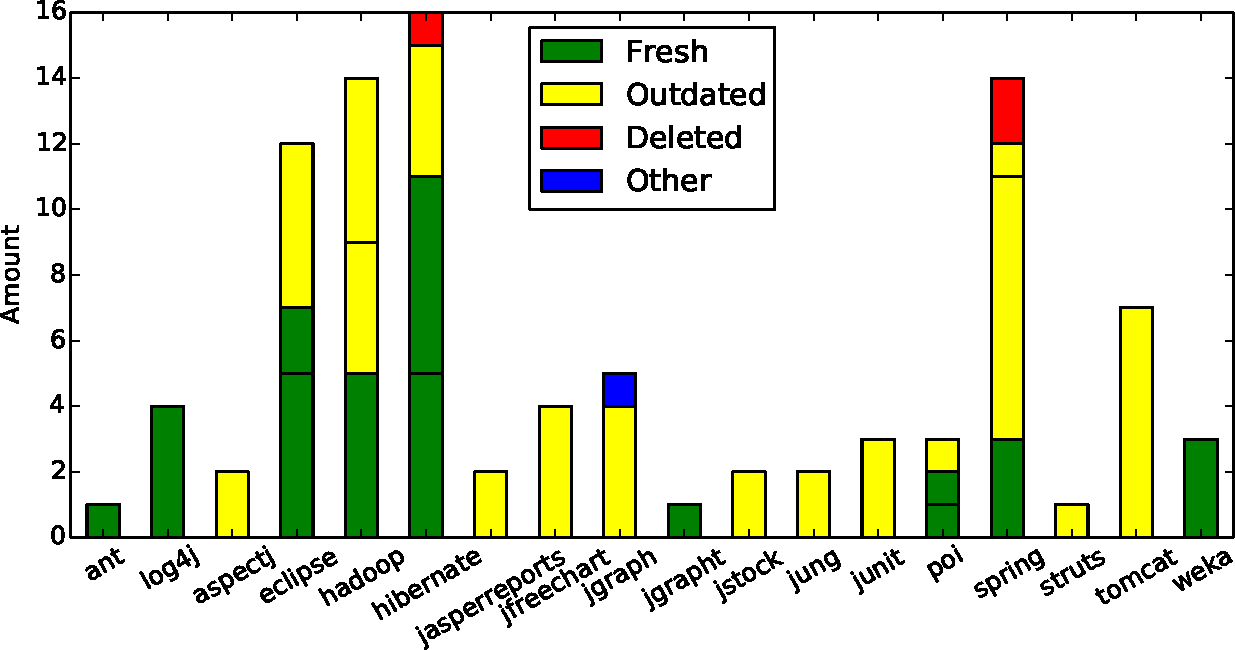
\includegraphics[width=0.8\linewidth]{outdated}
	\caption{Findings from outdated code investigation of 96 pattern-A online clone pairs}
	\label{fig:outdated}
\end{figure}

%\begin{table}
%	\centering
%	\caption{Breakdowns of findings from outdated code investigation of 96 category-A online clone pairs}
%	\label{tab:stale_code}
%	\small
%%	\resizebox{\columnwidth}{!}{%
%	\begin{tabular}{l|r|r|r|r|r}
%		\hline 
%		Project & Pairs & Outdated & Fresh & Del. & Others \\
%		\hline
%		ant & 1 & 0 & 1 & 0 & 0 \\
%		log4j & 4 & 0 & 4 & 0 & 0 \\
%		tomcat & 7 & 7 & 0 & 0 & 0 \\
%		aspectj & 2 & 2 & 0 & 0 & 0 \\
%		eclipse-SDK & 12 & 5 & 7 & 0 & 0 \\
%		hadoop & 14 & 9 & 5 & 0 & 0 \\
%		hibernate & 16 & 4 & 11 & 1 & 0 \\
%		jasperreports & 2 & 2 & 0 & 0 & 0 \\
%		jfreechart & 4 & 4 & 0 & 0 & 0 \\
%		jgraph & 5 & 4 & 0 & 0 & 1 \\
%		jgrapht & 1 & 0 & 1 & 0 & 0 \\
%		jstock & 2 &  2 & 0 & 0 & 0 \\
%		jung & 2 & 2 & 0 & 0 & 0 \\
%		junit & 3 & 3 & 0 & 0 & 0 \\
%		poi & 3 & 1 & 2 & 0 & 0 \\
%		spring & 14 & 9 & 3 & 2 & 0 \\
%		struts & 1 & 1 & 0 & 0 & 0 \\
%		weka & 3 & 0 & 3 & 0 & 0 \\
%		\hline
%		Total & 96 & 55 & 37 & 3 & 1 \\
%		\hline
%	\end{tabular} 
%%}
%\end{table}

\begin{table*}
	\centering
	\caption{58 code clones in Stack Overflow (SO) that were altered, rewritten, or removed from the project after posted and their respective licenses. Files can be changed ($C$) by modifications ($M$), deletion ($D$), and rewriting ($R$).}
	\label{tab:stale_code_details}
	\scriptsize
	\resizebox{2.1\columnwidth}{!}{%
	\begin{tabular}{r|l|c|p{4.5cm}|r|r|l|l|l|c|l}
		\hline 
		No. & Project & Ver. & File & Start & End & License & SO Post & License & $C$ & C$_{\textit{\textrm{date}}}$ \\
		\hline
			1 & \texttt{aspectj} & 1.6.9  & aspectjtools/../Agent.java  & 7 & 18 & -- & 18303692 & -- & $M$  & 2015-09-08 \\
			2 & \texttt{aspectj} & 1.6.9  & aspectjweaver/../Agent.java  & 7 & 18 & -- & 18303692 & & $M$  & 2015-09-08 \\
			3 & \texttt{eclipse-SDK} & & GenerateToStringAction.java  & 113 & 166 & EPLv1 & 2513183 & EPLv1 & $M$  &  2015-03-17 \\
			4 & \texttt{eclipse-SDK} & & GenerateToStringAction.java  & 117 & 126 & EPLv1  &  2513183	& EPLv1 & $M$  &  2015-03-17 \\
			5 & \texttt{eclipse-SDK} & & GenerateToStringAction.java  & 143 & 165 & EPLv1  &  2513183	& EPLv1 & $M$  &  2015-03-17 \\
			6 & \texttt{eclipse-SDK} & & GenerateToStringAction.java  & 178 & 187 & EPLv1  &  2513183	& EPLv1 & $M$  & 2011-03-01 \\
			7 & \texttt{eclipse-SDK} & & WizardDialog.java  & 377 & 394 & EPLv1  &   11861598	& -- & $M$  &  2011-02-03 \\
			8 & \texttt{hadoop} & 1.0.0 & DBCountPageView.java  & 275 & 287 & Apache-2 & 21702608 & -- & $M$  & 2011-06-12 \\
			9 & \texttt{hadoop} & 1.0.0 & DBCountPageView.java  & 289 & 309 & Apache-2 & 21702608 & -- & $M$  & 2011-06-12 \\
			10 & \texttt{hadoop} & 1.0.0 & JobSubmissionFiles.java  & 46 & 55 & Apache-2 & 14845581 & -- & $M$  & 2012-06-25 \\
			11 & \texttt{hadoop} & 1.0.0 & mapred/../LineRecordReader.java  & 47 & 60 & Apache-2 & 16180910 & -- & $M$  & 2011-07-25 \\
			12 & \texttt{hadoop} & 1.0.0 & mapreduce/../LineRecordReader.java  & 75 & 99 & Apache-2 & 16180910 & -- & $M$  & 2011-07-25 \\
			13 & \texttt{hadoop} & 1.0.0 & StringUtils.java  & 40 & 56 & Apache-2 & 801987 & -- & $M$  & 2013-02-04 \\
			14 & \texttt{hadoop} & 1.0.0 & TestJobCounters.java  & 186 & 192 & Apache-2 & 18833798 & -- & $M$  & 2011-06-12 \\
			15 & \texttt{hadoop} & 1.0.0 & TextOutputFormat.java  & 75 & 99 & Apache-2 & 16928749 & -- & $M$  & 2011-06-12 \\
			16 & \texttt{hadoop} & 1.0.0 & WritableComparator.java  & 44 & 54 & Apache-2 & 22315734 & -- & $M$  & 2014-11-20 \\
			17 & \texttt{hibernate} & 4.2.2 & ConnectionProviderInitiator.java  & 65 & 93 & -- & 15168494 & -- & $M$  & 2012-06-24 \\
			18 & \texttt{hibernate} & 4.2.2 & Example.java  & 224 & 243 & -- & 24924255 & -- & $M$  & 2013-04-23 \\
			19 & \texttt{hibernate} & 4.2.2 & SchemaUpdate.java  & 115 & 168 & -- & 23520731 & -- & $M$  & 2016-02-05 \\
			20 & \texttt{hibernate} & 4.2.2 & SettingsFactory.java  & 244 & 255 & -- & 8257554 & -- & $D$  & 2011-03-11 \\
			21 & \texttt{hibernate} & 4.2.2 & SQLServer2005LimitHandler.java  & 43 & 61 & -- & 23967852 & -- & $M$  & 2015-03-12 \\
			22 & \texttt{jasperreports} & 3.7.4 & JRVerifier.java  & 982 & 998 & LGPLv3+ & 8037824 & -- & $M$  & 2008-04-17 \\
			23 & \texttt{jasperreports} & 3.7.4 & JRVerifier.java  & 1221 & 1240 & LGPLv3+ & 8037824 & -- & $M$  & 2011-05-20 \\
			24 & \texttt{jfreechart} & 1.0.13 & AbstractXYItemRenderer.java  & 532 & 569 & LGPLv2.1+ & 12936580 & -- & $M$  & 2016-02-19 \\
			25 & \texttt{jfreechart} & 1.0.13 & KeyToGroupMap.java  & 18 & 30 & LGPLv2.1+ & 16058183 & -- & $M$  & 2013-07-03 \\
			26 & \texttt{jfreechart} & 1.0.13 & SpiderWebPlot.java  & 502 & 520 & LGPLv2.1+ & 21998949 & -- & $M$  & 2008-06-02 \\
			27 & \texttt{jfreechart} & 1.0.13 & SpiderWebPlot.java  & 522 & 536 & LGPLv2.1+ & 21998949 & -- & $M$  & 2008-06-02 \\
			28 & \texttt{jgraph} & 5.13.0.0 & HelloWorld.java  & 16 & 22 & LGPLv2.1+ & 6722760 & -- & $R$  & 2014-04-13 \\
			29 & \texttt{jgraph} & 5.13.0.0 & HelloWorld.java  & 28 & 40 & LGPLv2.1+ & 6722760 & -- & $R$  & 2014-04-13 \\
			30 & \texttt{jgraph} & 5.13.0.0 & HelloWorld.java  & 31 & 36 & LGPLv2.1+ & 6722760 & -- & $R$  & 2014-04-13 \\
			31 & \texttt{jgraph} & 5.13.0.0 & HelloWorld.java  & 39 & 56 & LGPLv2.1+ & 6722760 & -- & $R$  & 2014-04-13 \\
			32 & \texttt{jstock} & 1.0.7c & GoogleMail.java  & 18 & 42 & GPLv2+ & 14940863 & -- & $M$  & 2015-12-13 \\
			33 & \texttt{jstock} & 1.0.7c & GoogleMail.java  & 18 & 42 & GPLv2+ & 24680923 & -- & $M$  & 2015-12-13 \\
			34 & \texttt{jung2} & 2\_0\_1  & ShortestPathDemo.java  & 106 & 117 & -- & 6025026 & -- & $M$  & 2010-04-13 \\
			35 & \texttt{jung2} & 2\_0\_1  & ShortestPathDemo.java  & 158 & 172 & -- & 6025026 & -- & $M$  & 2010-04-13 \\
			36 & \texttt{junit} & 4.11 & Assert.java  & 33 & 52 & -- & 23586872 & -- & $M$  & 2015-05-12 \\
			37 & \texttt{junit} & 4.11 & ExternalResource.java  & 4 & 23 & -- & 7504040 & -- & $M$  & 2016-06-25 \\
			38 & \texttt{junit} & 4.11 & ExpectException.java  & 11 & 29 & -- & 8802082 & -- & $M$  & 2014-05-26 \\
			39 & poi & 3.6 & WorkbookFactory.java  & 18 & 28 & Apache-2 & 12593810 & -- & $M$  & 2015-04-29 \\
			40 & \texttt{spring} & 3.0.5 & AnnotationMethodHandler \newline ExceptionResolver.java  & 224 & 233 & Apache-2 & 5660519 & -- & $D$  & 2012-01-20 \\
			41 & \texttt{spring} & 3.0.5  & AutowireUtils.java  & 32 & 42 & Apache-2 & 20913543 & -- & $M$  & 2014-10-28 \\
			42 & \texttt{spring} & 3.0.5  & CustomCollectionEditor.java  & 33 & 71 & Apache-2 & 18623736 & -- & $M$  & 2013-11-21 \\
			43 & \texttt{spring} & 3.0.5  & DefaultAnnotation \newline HandlerMapping.java  & 78 & 92 & Apache-2 & 3758110 & -- & $D$  & 2012-01-20 \\
			44 & \texttt{spring} & 3.0.5  & DefaultPropertiesPersister.java  & 69 & 80 & Apache-2 & 6149818 & -- & $M$  & 2013-03-19 \\
			45 & \texttt{spring} & 3.0.5  & org.springframework.test/../ \newline DelegatingServletInputStream.java  & 6 & 20 & Apache-2 & 20996373 & -- & $M$  & 2016-07-15 \\
			46 & \texttt{spring} & 3.0.5  & org.springframework.web/../ \newline DelegatingServletInputStream.java  & 6 & 20 & Apache-2 & 20996373 & -- & $M$  & 2008-12-18 \\
			47 & \texttt{spring} & 3.0.5  & org.springframework.web.servlet/../ \newline DelegatingServletInputStream.java  & 6 & 20 & Apache-2 & 20996373 & -- & $M$  & 2008-12-18 \\
			48 & \texttt{spring} & 3.0.5  & DispatcherServlet.java  & 91 & 103 & Apache-2 & 4781746 & -- & $M$  & 2011-08-08 \\
			49 & \texttt{spring} & 3.0.5  & Jaxb2Marshaller.java  & 253 & 269 & Apache-2 & 10924700 & -- & $M$  & 2012-08-28 \\
			50 & \texttt{spring} & 3.0.5  & ScheduledTasksBean \newline DefinitionParser.java  & 42 & 52 & Apache-2 & 3751463 & -- & $M$  & 2016-07-05 \\
			51 & \texttt{struts2} & 2.2.1  & DefaultActionMapper.java  & 91 & 103 & Apache-2 & 14019840 & -- & $M$  & 2013-10-18 \\
			52 & \texttt{tomcat} & 7.0.2  & BasicAuthenticator.java  & 25 & 73 & Apache-2 & 21734562 & -- & $M$  & 2016-08-04 \\
			53 & \texttt{tomcat} & 7.0.2  & BasicAuthenticator.java  & 33 & 43 & Apache-2 & 21734562 & -- & $M$  & 2016-08-04 \\
			54 & \texttt{tomcat} & 7.0.2  & CoyoteAdapter.java  & 543 & 553 & Apache-2 & 24404964 & -- & $M$  & 2012-11-18 \\
			55 & \texttt{tomcat} & 7.0.2  & CoyoteAdapter.java  & 557 & 573 & Apache-2 & 24404964 & -- & $M$  & 2012-11-18 \\
			56 & \texttt{tomcat} & 7.0.2  & FormAuthenticator.java  & 51 & 61 & Apache-2 & 21734562 & -- & $M$  & 2016-08-04 \\
			57 & \texttt{tomcat} & 7.0.2  & HttpServlet.java  & 111 & 124 & Apache-2 & 5266856 & -- & $M$  & 2011-10-22 \\
			58 & \texttt{tomcat} & 7.0.2  & JspRuntimeLibrary.java  & 252 & 296 & Apache-2 & 10289462 & -- & $M$  & 2012-09-12 \\
		\hline
	\end{tabular} %
}
\end{table*}

\subsection{RQ4: Software Licensing Violation}
Software licensing plays an important role in software development. Violation of software licenses impacts software delivery and also leads to legal issues \cite{Sprigman2015}. 
%It is an emerging area that software engineering research community is paying attention to. For example, 
One can run into licensing issue if they do not check before integration third-party source code into their software. A study by An et al.~\cite{An2017} found 1,219 cases of potential license violations between 399 Android apps and Stack Overflow code. %there are studies of automatic technique to identify software licensing from source code files \cite{German2010} 

\begin{table}
	\centering
	\caption{14 Qualitas projects with the highest number of true clones on Stack Overflow with their respective licenses}
	\label{t:q_projects_license}
	%	\resizebox{\columnwidth}{!}{%
	\small
	\begin{tabular}{l|r|p{4cm}}
		\hline 
		Project & Version & Licenses (no.~of files) \\
		\hline
		%		apache-ant & 1.8.4 & Apache2.0 \\
		%		apache-log4j & 1.2.16 & \\
		aspectj & 1.6.9 & Apache-1.1 (182), CPLv1 (3), \newline EPLv1 (2011), None (23), \newline SeeFile (6), Unknown (286) \\
		\hline
		eclipse-SDK &  4.1 & Apache-2 (2183), \newline BSD3NoWarranty (107), \newline CDDLorGPLv2 (296), \newline EPLv1 (18823), MPLv1.1 (93), \newline None (224), SeeFile (8), \newline spdxBSD3 (185), \newline spdxMIT (1), Unknown (714) \\
		\hline
		hadoop & 1.0.0 & Apache-2 (1,935), \newline spxdBSD/Apache-2 (8) \newline None (33), Unknown (14) \\
		\hline
		hibernate & 4.2.2 & Apache-2 (20), \newline LGPLv2.1+ (31) \newline PublicDomain (1), \newline None (1,850), SeeFile (4), \newline Unknown (4,324) \\
		\hline
		jasperreports & 3.7.4 & LGPLv2.1+ (3), \newline LGPLv3+ (1,581), \newline None (1), Unknown (4)\\
		\hline
		jfreechart & 1.0.13 & LGPLv2.1+ (989) \\
		\hline
		jgraph & 5.13.0.0 & LGPLv2.1+ (4), \newline spdxBSD (2), Unknown (151), \newline None (24), SeeFile (9) \\
		\hline
		%		jgrapht & 0.8.1 & LGPL 2.1 \& Eclipse  1.0 \\
		jstock & 1.0.7c & LGPLv2.1+ (1), \newline GPLv2+ (239), \newline Apache-2 (1), BSD3 (1), \newline None (23), SeeFile (1), \newline spdxMIT (3), Unknown (5)\\
		\hline
		jung2 & 2-0-1 & N/A \\
		\hline
		junit & 4.11 & None (160), Unknown (4)  \\
		\hline
		poi & 3.6 & Apache-2 (2,002), None (5) \\
		\hline
		spring & 3.0.5 & Apache-2 (2,982) \\
		\hline
		struts2 & 2.2.1-all & Apache-2 (1,717), \newline spdxBSD3 (6), \newline None (118), SeeFile (1), \newline Unknown (2) \\
		\hline
		tomcat & 7.0.2 & Apache-2 (1,313), None (11) \\
		%		weka & 3-7-9 & \\
		\hline
	\end{tabular} %
	%	}
\end{table}

\begin{table}[]
	\centering
	\caption{Licenses of 523 clone pairs in category A, B, and C}
	\label{tab:license_abc}
	\small
	\resizebox{\columnwidth}{!}{%
	\begin{tabular}{p{1.5cm}|l|p{2.2cm}|r|r|r}
		\hline
		Type                                           & SO          & Qualitas          	& A & B & C \\
		\hline
		No license \newline (\textit{NL})  & None        & None           &  18 & 62 & 5 \\
		\hline
		Compatible  							 & Apache2     & Apache2  	   &  0 & 1 & 0 \\
		License	   						             & EPLv1       & EPLv1                 &  14 &  6 & 0 \\
		(\textit{CL})													& None        & CC BY 3.0   &  0 & 12 & 0 \\
		\hline
	    Incompat. 								   & None       & Apache2  						& 41 & 29 & 3 \\
		License								         & None        & BSD/BSD3                      & 0 & 64 & 0 \\
		(\textit{IL}) 								 & None        & CDDLorGPLv2                & 0 & 63 & 4 \\
															& None        & EPLv1                               & 0 & 33 & 0\\
															& None        & GPLv2/2+/3+                  &  5 & 52 & 14 \\
															& None        & LGPL2.1+/3+                   &  18 & 33 & 2 \\
															& None        & AGPLv3/3+                     & 0 & 9 &1  \\
															& None        & MPLv1\_1                         & 0 & 1 & 0\\
															& None        & spdxBSD3                      & 0 & 8 & 1 \\
															& None        & Unidentifiable                 & 0 & 1 & 0 \\
															& Proprietary & None                            & 0 & 21 & 1 \\
															& BSD3        & GPLv2+							& 0 & 1 & 0 \\
		\hline
		\multicolumn{3}{l|}{Total} 	       																&  96 & 396 & 31 \\
		\hline
	\end{tabular} %
}
\end{table}

\begin{figure*}
	\minipage{0.32\textwidth}
	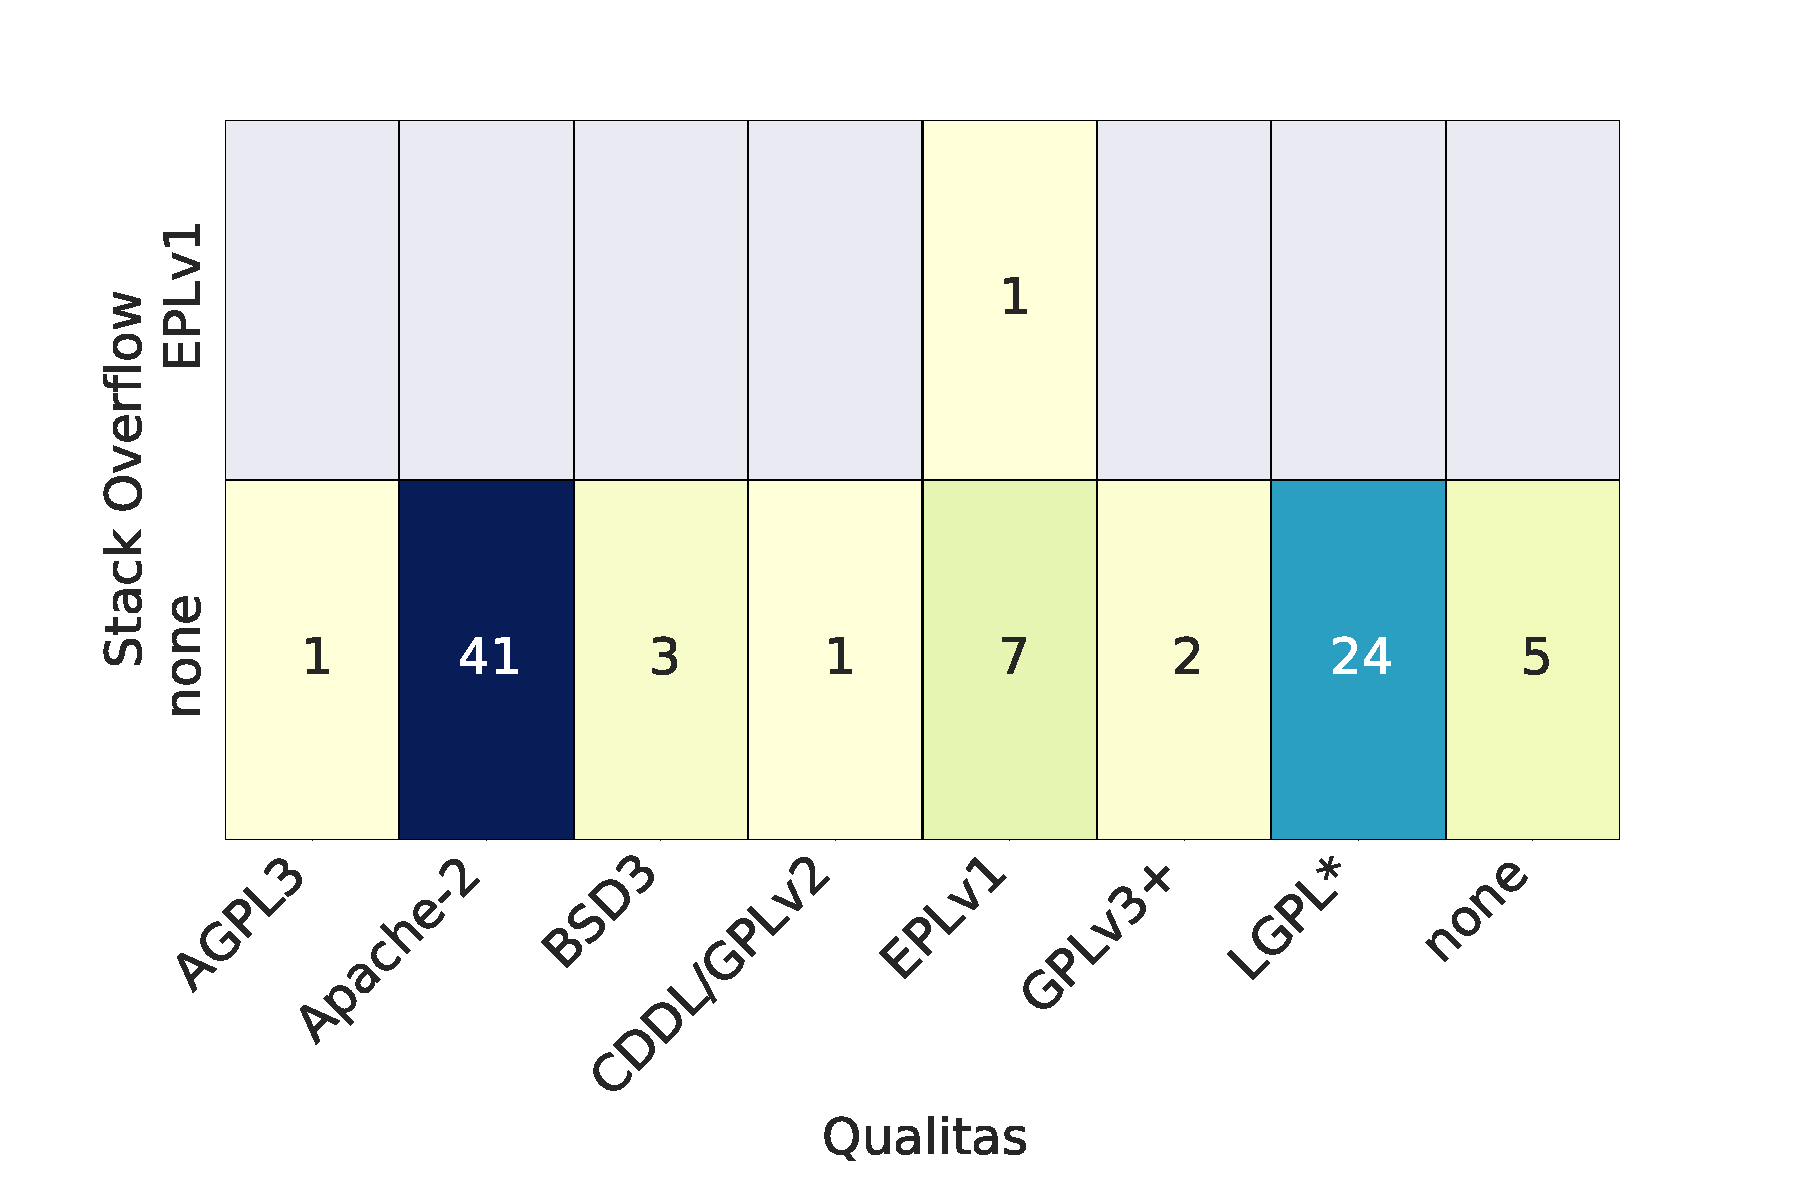
\includegraphics[width=\linewidth]{heatmap_a}
	\caption*{(1) category A}\label{fig:heatmap_a}
	\endminipage\hspace{0.3cm}
	\minipage{0.32\textwidth}
	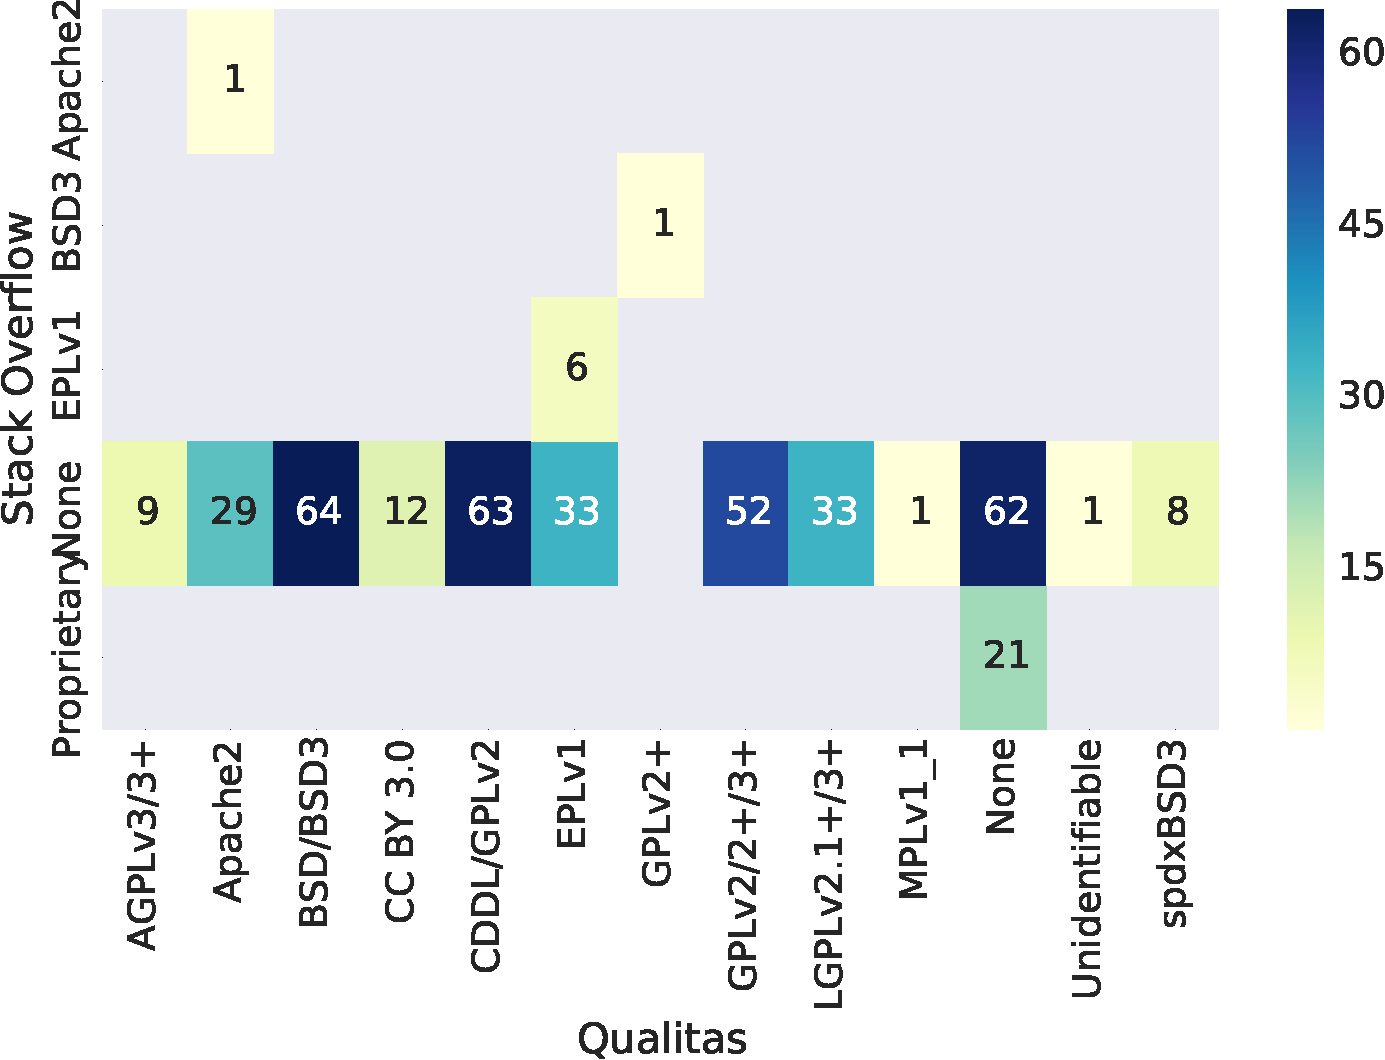
\includegraphics[width=\linewidth]{heatmap_b}
	\caption*{(2) category B}\label{fig:heatmap_b}
	\endminipage\hfill
	\minipage{0.32\textwidth}%
	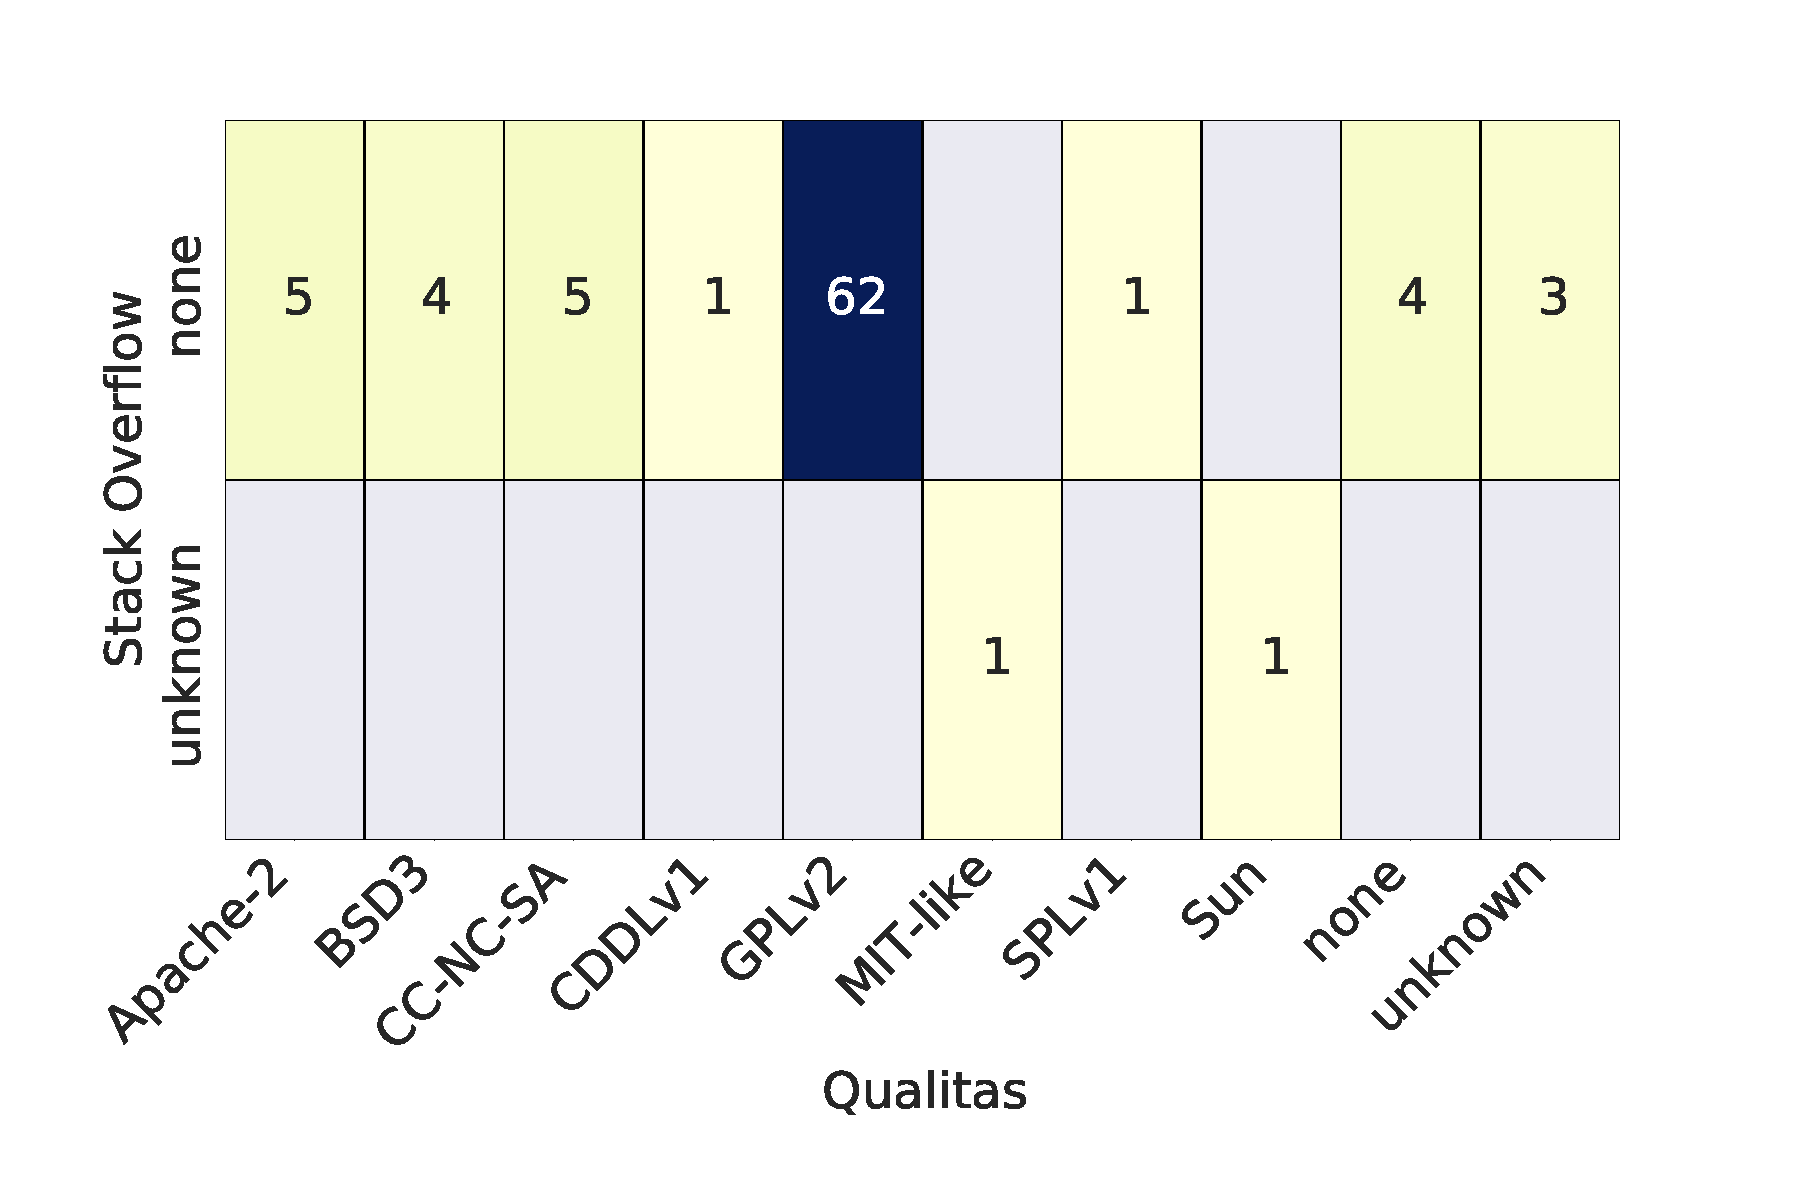
\includegraphics[width=\linewidth]{heatmap_c}
	\caption*{(3) category C}\label{fig:heatmap_c}
	\endminipage
	\caption{Licensing between Stack Overflow code snippets and Qualitas Java file of 523 true online clone pairs}
\end{figure*}

In our study, we reveal another possible situation of software licensing issues caused by code cloning ``to Stack Overflow''. We found with evidence that 96 pieces of code had been copied from 14 Qualitas projects to Stack Overflow as code examples. They are also marked as accepted answers which increased their chances of being reused. The 14 open source projects came with their respective software licenses (shown in \Cref{t:q_projects_license}). However, the licensing information were mostly missing from these clones after they were posted on Stack Overflow. The licensing terms on the top of source code are not copied because mostly a small part of the file was cloned to Stack Overflow. If developers copy and reuse these licensed pieces of code in their projects, conflicts may happen without their realisation. 

The summary of licensing information is listed in \Cref{tab:license_abc}. The licenses were extracted by Ninka, an automatic license identification tool \cite{German2010}. For the ones that could not be automatically identified by Ninka and had been reported as \texttt{SeeFile} and \texttt{Unknown}, we looked at them manually.  The table shows license of Stack Overflow snippets (denoted as SO) and Qualitas source code. The number of clone pairs of each license matching has been grouped according to online cloning patterns QS, UD, and ES. In overall, we can see that most of the Stack Overflow snippets do not have licensing terms with them while their clone counterparts in Qualitas project do. 

\textbf{No license or compatible license:} There are 85 \textit{NL} clone pairs which do not have licensing information (None vs.~None) and 13 pairs in type \textit{CL} which have compatible licenses (Apache2 vs.~Apache2; EPLv1 vs.~EPLv1; None vs.~CC BY 3.0). They are safe for being reused. Since source code and text on Stack Overflow posted before 1st March 2016 are protected by CC BY 3.0 (and MIT license from 1st March 2016 onwards), we can treat Stack Overflow code snippets without licensing information as having CC BY 3.0 by default. CC BY 3.0 license is relaxed and it only request attribution when reuse. 

\textbf{Incompatible license:} there are a large number of clone pairs in type \textit{IL} which do not contain licensing information after they are posted on Stack Overflow or having different license that its Qualitas clone counterpart. 96 category-A clones are the pairs that we have evidence of being copied from Qualitas to Stack Overflow. 64 of them do not contain licensing terms after posted and are controversial for being reused. 396 clone pairs in category B are highly similar clones that we do not have evidence of copying. 315 of them have incompatible licenses. Interestingly, there are 21 clone pairs that Stack Overflow snippets contain Sun and MIT-like license while Qualitas clones do not have any license information. There is also one clone pair having BSD3 license on Stack Overflow while having GPLv2+ in Qualitas source code. Lastly, 26 out of 31 clone pairs in category C have incompatible license. They are clones that have been identified to be copied from an external source. Again, most of the clones in Qualitas contain license while the Stack Overflow snippets do not. 

\textbf{For RQ4, we observed xx code snippets on Stack Overflow that violate the license of their original software. Most of them do not contain licensing statements after copied to Stack Overflow. \FIXME{More}}

\subsubsection{Interesting Finding: External Clones}

\begin{table}[]
	\centering
	\caption{31 external clones found in Stack Overflow posts}
	\label{tab:ext_clones}
	\begin{tabular}{l|r|r}
		\hline
		Type        & FOSS & Web \\ \hline
		StackOverflow only     & 1    & 1   \\
		StackOverflow + Qualitas & 15   & 14  \\ \hline
	\end{tabular}
\end{table}

We found 31 clone pairs which either clones from Stack Overflow side or from both sides are found to be a copy of code snippet from somewhere else besides Qualitas projects. This complements the findings of inter clones between software projects \cite{Svajlenko2014} by showing that clones can also be copied over different websites on the Internet. There are 15 clone pairs that are originated from programming websites. For example, we found a clone of code snippet to convert numbers into words which is copied from \url{http://www.rgagnon.com/javadetails/java-0426.html}. Both Stack Overflow and \textit{Compiere} project source code contain attribution to the original source. Another example is a code of algorithm to generate graphical \textit{Perlin noise} copied from \url{http://mrl.nyu.edu/~perlin/noise/}. This code is used in both Stack Overflow and \textit{AoI} project with attribution. The original code of the 15 clone pairs do not have licensing information so these clones do not violate any license. However, there are 4 clone pairs that are cloned from \textit{JUnit} to both Stack Overflow and \textit{Eclipse} and 12 pairs cloned from other Java projects outside Qualitas corpus. They are originated from \textit{zxing} projects, Apache projects (ant, jasper), Java packages (\texttt{java.util}, \texttt{javax.servlet}, JUnit, and \texttt{org.bouncycastle.crypto} project.

\section{Threats to Validity}

\section{Related Work}

\textbf{Stack Overflow} is a gold mine for software engineering research. Its rich and developer-driven data are invaluable. Since posts on Stack Overflow may contain code snippets embedded within natural language text, they become a huge database for source code and code-relevant information. The Stack Overflow data set has been put to use in several previous studies. In terms of developer-assisting tools, Seahawk is an Eclipse plug-in that searches and recommends relevant code snippets from Stack Overflow \cite{Ponzanelli2013}. A follow up work, Prompter, by Ponzanelli et al.~\cite{Ponzanelli2014} achieves the same goal but with improved algorithms. The code snippets on Stack Overflow are mostly examples or solutions to programming problems. Hence, several code search systems use whole or partial data from Stack Overflow as their code search databases \cite{Diamantopoulos2015,Keivanloo2014,Park2014, Stolee2014,Subramanian2013,Diamantopoulos2015}. Furthermore, Treude et al.~use machine learning techniques to extract insight sentences from Stack Overflow and use them to improve API documentation \cite{Treude2016}.

Another aspect is knowledge extraction from Stack Overflow. Nasehi et al.~studied what makes a good code example by analysing answers from Stack Overflow \cite{Nasehi2012}. Similarly, Yang et al.~\cite{Yang2016} analysed Stack Overflow snippets across various programming languages and observed that code snippets in Python and Javascript are the most usable. Wang et al.~\cite{Wang2013_StackOverflow} use Latent Dirichlet Allocation (LDA) topic modelling to analyse questions and answers from Stack Overflow so that they can automatically categorise new questions. There are also studies trying to understand developers' behaviours on Stack Overflow, e.g.~\cite{Movshovitz-Attias2013,Rosen2016,Choetkiertikul2015,Bosu2013}, while some studies aim to improve Stack Overflow itself \cite{Diamantopoulos2015, Wang2014}. 

\textbf{Code clone detection} is a long-standing research topic in software engineering. Whether clones are good or bad for software is still controversial \cite{Sajnani2016,Kapser2003,Kapser2008,Krinke2008,Hotta2010,Gode2011,Harder2013}. However, by only knowing how many code clones residing in software and how they evolve \cite{Pate2013,Mondal2011} can provide several valuable insights into the software systems. Besides clones, clone detection has its several applications such as software plagiarism detection~\cite{Prechelt2002}, 
source code provenance~\cite{Davies2013}, and software licensing conflicts~\cite{German2009}.

Two code fragments are clones if they are similar enough according to a given definition of similarity \cite{Bellon2007}. Given an open interpretation of ``definition of similarity'', there are various clone detection tools and their siblings, code plagiarism detectors, invented based on plethora of different code similarity measurements \cite{Roy2008, Ragkhitwetsagul2016,Svajlenko2014}. Some tools
use string comparison techniques such as Simian \cite{simian}. NiCad \cite{Roy2008,Cordy} also exploits Longest Common Subsequence (LCS) string similarity measure to discover clones after applying code pretty-printing using TXL \cite{Cordy2006}. Many tools do not work on original source code directly but transform them into an
intermediate representation such as tokens and apply similarity
measurement on them. These tools include SourcererCC~\cite{Sajnani2016}, CCFinder~\cite{Kamiya2002},
CP-Miner~\cite{Li2006}, iClones~\cite{Gode2009} and a few more~\cite{Burrows2007, Smith2009, Duric2012, Prechelt2002, Schleimer2003}. 
To find more challenging clones such as clones with added/deleted/reordered statements or equivalent loop and conditional statements (i.e.~type-3 clones), structural similarity of clones is needed.
This structural similarity can be discovered by comparing AST as found in CloneDR~\cite{Baxter1998} and Deckard~\cite{Jiang2007a} or by using program dependence
graphs~\cite{Krinke2001,Komondoor2001}. 

Kapser et al.~studied clones in Linux file systems and create 11 patterns of code cloning based on four groups: Forking, Templating, Customization and Exact match~\cite{Kapser2003,Kapser2008}. Our study partially adapted their patterns for our online code clone classification scheme.

\textbf{Clone agreement} is useful in when clone oracle is absent. Since clone detectors are different in their detection approaches, they may behave differently and report different clones even on the same data set. Some researchers exploit these different behaviours of clone detectors by finding their agreement and obtain highly-confident clones \cite{Bellon2007,Wang2013}. Using the same data set, clone pairs that are agreed by several tools (or several code similarity measurement techniques) are highly potential to be true clones than the ones reported by only a single tool \cite{Wang2013,cr2016ssbse,Funaro2010}. These studies also report that sensitivities of the tools' parameter settings have strong effects to the results \cite{Wang2013,cr2016ssbse}.

\textbf{Software licensing} is crucial for open source and industrial software development. Di Penta et al.~study an evolution of software licensing in six FOSS and found that licensing statements change over time \cite{DiPenta2010}. German et al.~\cite{German2009} performed an empirical study of code siblings (code clones among different systems coming from the same source) and found that licensing conflicts can occur between the clone siblings. Later, German et al.~\cite{German2010} created Ninka, a tool to automate identification of software license from program source code. We use Ninka to analyse software license from Stack Overflow snippets and Qualitas projects. 

\textbf{Reusing of outdated third-party source code} occurs in software development. Xia et al.~\cite{Xia2014} show that a large number of open source systems reuse outdated third-party libraries from famous open source projects. Using outdated code give detrimental effects to the software since they may introduce vulnerabilities. Our study discovers similar findings in the context of outdated code from Stack Overflow.

The work that is closely similar to us is a study by An et al.~\cite{An2017}. The authors investigated clones between 399 Android apps and Stack Overflow posts. They found 1,226 code snippets which were reused from 68 Android apps. They also observed that there are 1,219 cases of potential license violations. However, the authors rely on the timestamp to judge whether the code has been copied from/to Stack Overflow along with confirmations from six developers. Instead of Android apps, we investigated clones between Stack Overflow and 111 open source projects. Our results confirm their findings that there are clones from software projects to Stack Overflow with potential licensing violations. In our work, we defined seven patterns of online code cloning and performed a large-scale manual check of 3,450 clone pairs. We discovered 96 clone pairs with strong evidences, based on natural text in comments and post contents, that they were copied from Qualitas to Stack Overflow. By comparing the clones to their latest versions in the software, we found that 58 code snippets on Stack Overflow are outdated and harmful for reuse.

\section{Conclusions}
This paragraph will end the body of this sample document.
Remember that you might still have Acknowledgments or
Appendices; brief samples of these
follow.  There is still the Bibliography to deal with; and
we will make a disclaimer about that here: with the exception
of the reference to the \LaTeX\ book, the citations in
this paper are to articles which have nothing to
do with the present subject and are used as
examples only.
%\end{document}  % This is where a 'short' article might terminate

%ACKNOWLEDGMENTS are optional
\section{Acknowledgments}
This section is optional; it is a location for you
to acknowledge grants, funding, editing assistance and
what have you.  In the present case, for example, the
authors would like to thank Gerald Murray of ACM for
his help in codifying this \textit{Author's Guide}
and the \textbf{.cls} and \textbf{.tex} files that it describes.

\begin{figure}
	\centering
	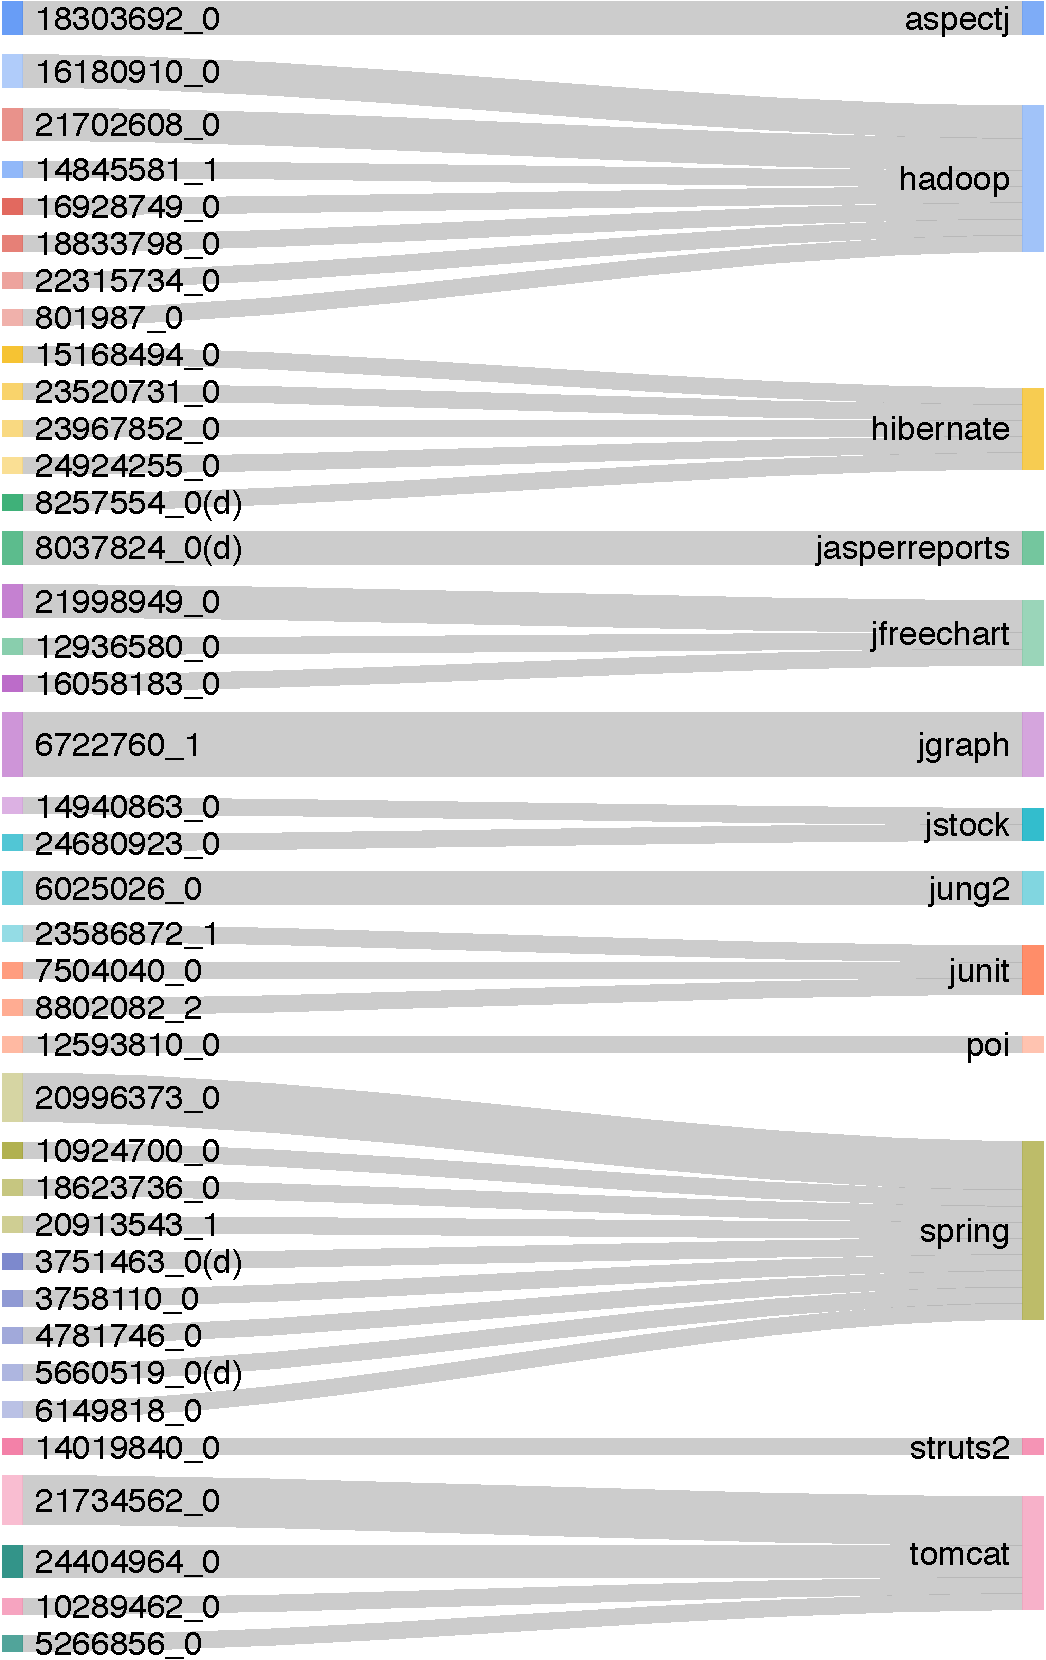
\includegraphics[width=\linewidth]{Sankey_proj}
	\caption{Relationships of 58 Stack Overflow clone pairs to their original projects. 55 are outdated and 3 are deleted (shown using (d) suffix).}
	\label{fig:sankey}
\end{figure}

%
% The following two commands are all you need in the
% initial runs of your .tex file to
% produce the bibliography for the citations in your paper.
\bibliographystyle{abbrv}
\bibliography{sigproc}  

\end{document}
